% The preamble has been dumped out as out/presentationpreamble.fmt file. You can recreate that file by
% xelatex -ini -jobname="pinholepreamble" -output-directory=out "&xelatex pinholepreamble.tex\dump"
% 
% To compile you need to load that binary file using -fmt option
% xelatex -fmt out/pinholepreamble.fmt -output-directory=out pinhole.tex
%\documentclass[10pt, compress]{beamer}
\usetheme{m}
 
 \usepackage{booktabs} % for better tables
 \usepackage{media9} % for includemedia i.e. videos
 \usepackage{xcolor} % for more colors
 \usepackage{hyperref} % for links
 \usepackage{cutwin} % text wrapped around figures
 \usepackage[backend=bibtex]{biblatex} % fancy citations
 \usepackage{ifthen}
 
\usepackage{tikz}
\usetikzlibrary{shadows,trees}
\usetikzlibrary{shapes,calc,backgrounds}
\usetikzlibrary{intersections}
\usepgfplotslibrary{dateplot}


%\tikzset{external/system call={xelatex -fmt out/pinholepreamble.fmt \tikzexternalcheckshellescape -shell-escape -halt-on-error -interaction=batchmode -jobname "\image" "\texsource"}}
%

% transparency
%\setbeamercovered{transparent=15}

\title{Computer Imaging: Build Your Own Camera}
\date{\today}
\author{Vikas Dhiman\\ David Johnson\\ Jason J Corso}
\institute{University of Michigan}
\bibliography{pinhole}

\begin{document}
\maketitle
\begin{frame}{Contents}
  % This slide will be removed later
  \tableofcontents
\end{frame}

\section{Modern Cameras}
\begin{frame}{Modern cameras}
    \includemedia[label=high-fps-camera,
      width=\linewidth,height=0.5\linewidth, % 16:9
      activate=pageopen,
      addresource=media/bullet-time.mp4,
      flashvars={
        source=media/bullet-time.mp4
        &loop=false             % loop video
        &scaleMode=letterbox   % preserve aspect ratio while scaling the video
      }
    ]{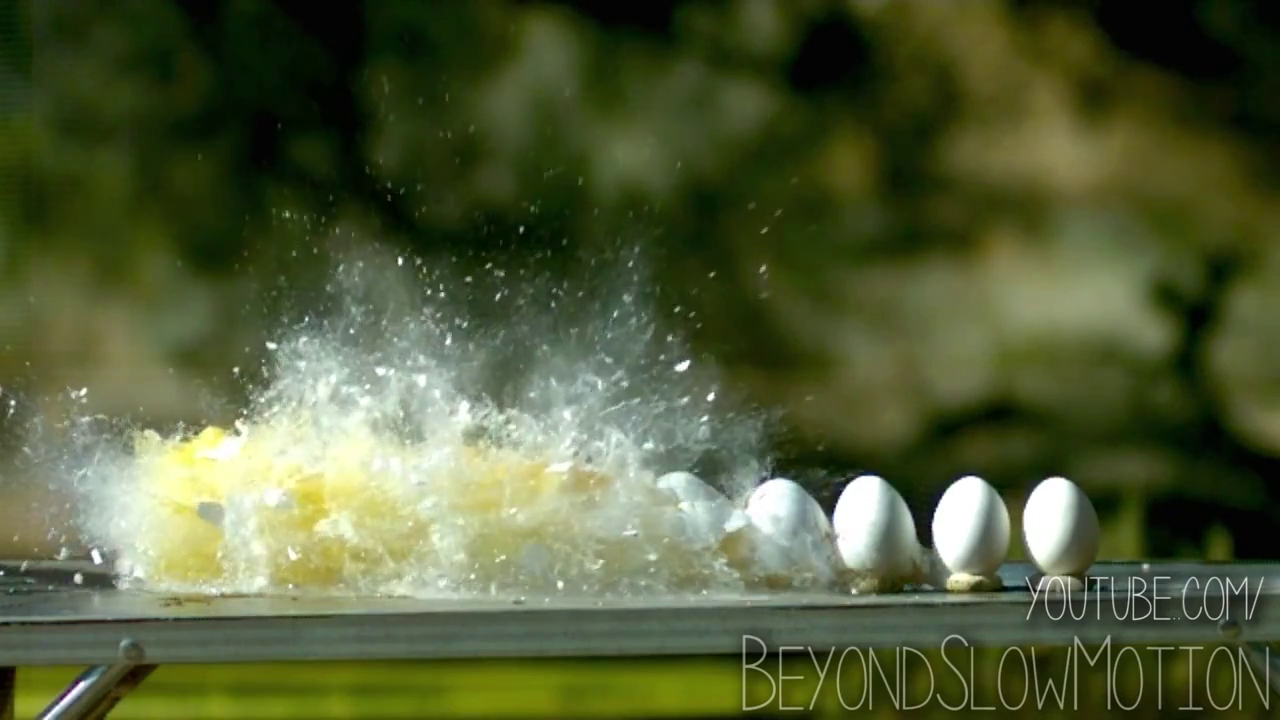
\includegraphics[width=\textwidth]{media/bullet-time.png}}{VPlayer.swf}
\end{frame}

\begin{frame}{Modern cameras}
    \includemedia[label=matrix-bullet-time-shot,
      width=\linewidth,height=0.6\linewidth, % 16:9
      activate=pageopen,
      addresource=media/bullet-time-shot.mp4,
      flashvars={
        source=media/bullet-time-shot.mp4
        &loop=false             % loop video
        &scaleMode=letterbox   % preserve aspect ratio while scaling the video
      }
    ]{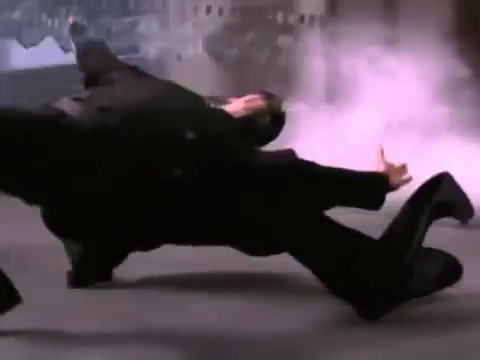
\includegraphics[width=\textwidth]{media/bullet-time-shot.png}}{VPlayer.swf}
\end{frame}
% \begin{frame}{Sources}
%   \begin{itemize}
%     \item 
%       \url{http://www.exploratorium.edu/science_explorer/pringles_pinhole.html}
%     \item
%       \url{http://www.learner.org/workshops/sheddinglight/}
%   \end{itemize}
% \end{frame}
% \begin{frame}{Pinhole camera}
%   \centering
%   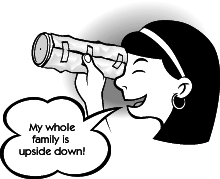
\includegraphics{media/girl_looks.png}
% \end{frame}

\section{About Light}
% Interesting notes/facts/videos about how human eye works.
% First camera "possibly" developed by ancient greeks and ancient Chinese.
% First documented description of a camera dates back to 1021 AD by a Arab physicist Ibn al-Haytham in his "Book of optics"
%%
%% How do you think our eyes work?
%% 
%% 
%% or 
%% 
%% 
% Rhetoric questions? Get kids involved
% What do kids think, how does eye/camera work?
\begin{frame}{How do we see things?}
  
  \begin{tikzpicture}[scale=0.5]
    \path [use as bounding box] (-4,0) rectangle (11,13);
    \node [anchor=south](tree) at (0,0) {
\includegraphics[width=7cm]{media/tree.png}};
    \node [anchor=south] (boy) at (10,1) {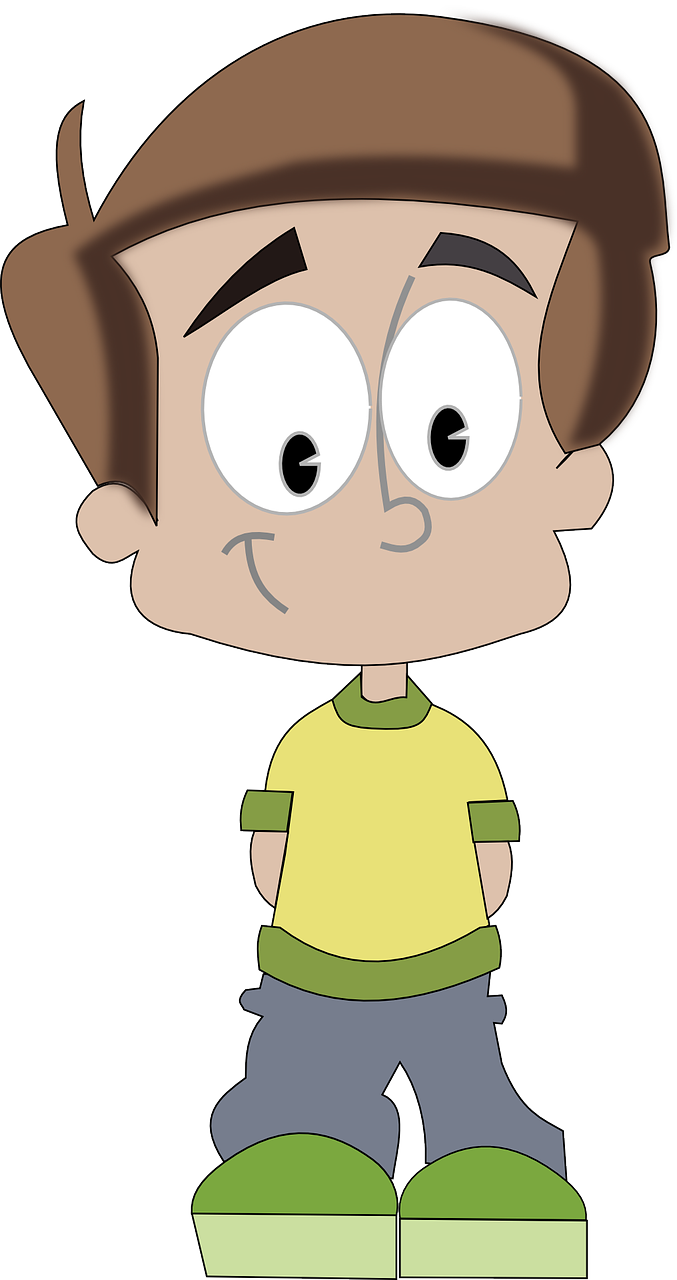
\includegraphics[width=1cm]{media/boy.png}};
    \coordinate (sun) at (7,12);
    \visible<2->{
      \fill [yellow] (sun) circle (1);
    }
    \visible<3->{
      \foreach \y in {10, 20, 30} 
      {
        \draw [very thick,yellow] ($(sun) + (-150+\y:1.1)$) -- ($(tree) + (80-2*\y:3)$) node [inner sep=0] (trays) {};
        \draw[very thick, green] (trays)-- ($(boy)+(0,0.6)$);
      }
    }
  \end{tikzpicture}

\end{frame}


\begin{frame}{How do we see things?}
  \begin{columns}
    \begin{column}{0.7\textwidth}
      \begin{itemize}
        \item
          Does the ``sight'' travel from our eyes to the object?\\
          \visible<2-> {\color{red}Euclid other Greek philosophers believed so around 300 BC}
       \item
         \color{black}{or the ``light'' travels from the object to our eyes?}\\
         \visible<3-> {\color{red}Modern scientists the believe so.}
      \end{itemize}
    \end{column}
    \hspace{-2cm}
    \begin{column}{0.3\textwidth}
      \centering
        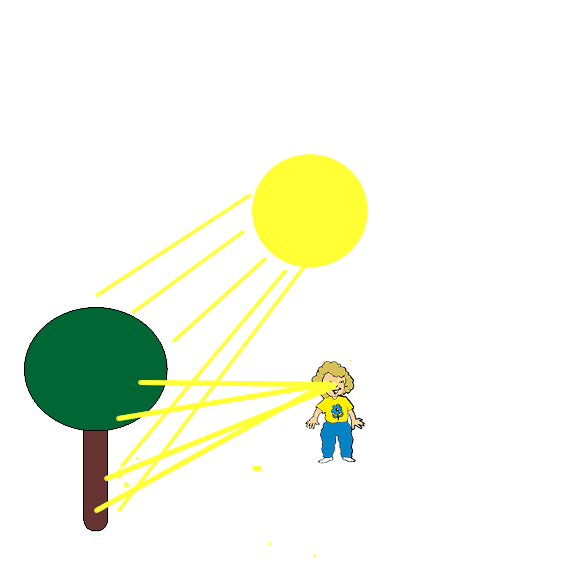
\includegraphics[width=1.4\textwidth]{media/lghtmisc2.pdf}
    \end{column}
  \end{columns}
\end{frame}
% 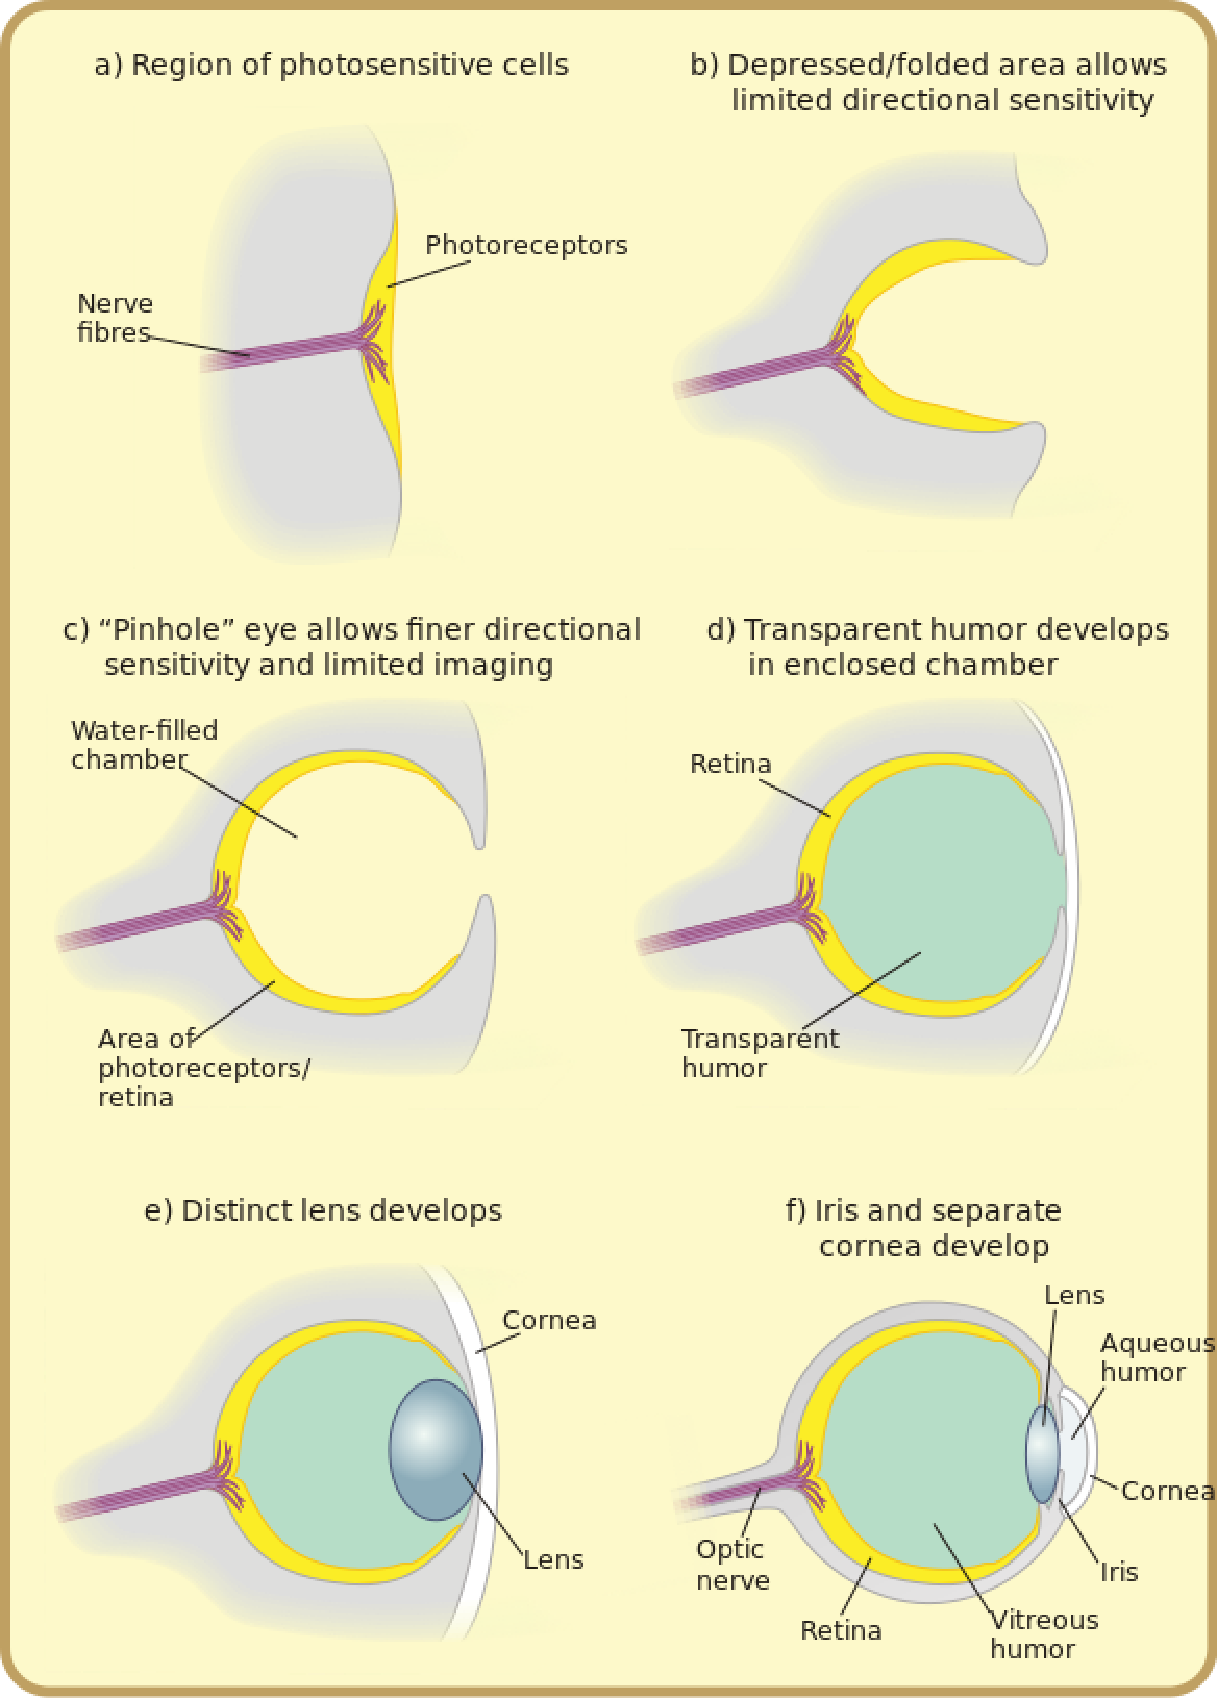
\includegraphics[width=\textwidth]{media/Diagram_of_eye_evolution.svg}
% \footfullcite{}

% \begin{frame}{What does it mean to see things?}
% 
% \end{frame}

\begin{frame}{What is light?}
  \begin{columns}
    \begin{column}{0.7\textwidth}
      \begin{itemize}
        \item Greek philosophers believed that sight was possible because of interaction of fire in eyes and in the sun.
        \item Euclid, a Greek philosopher, gave  us some particular insights about light.
      \end{itemize}
    \end{column}
    \begin{column}{0.3\textwidth}
      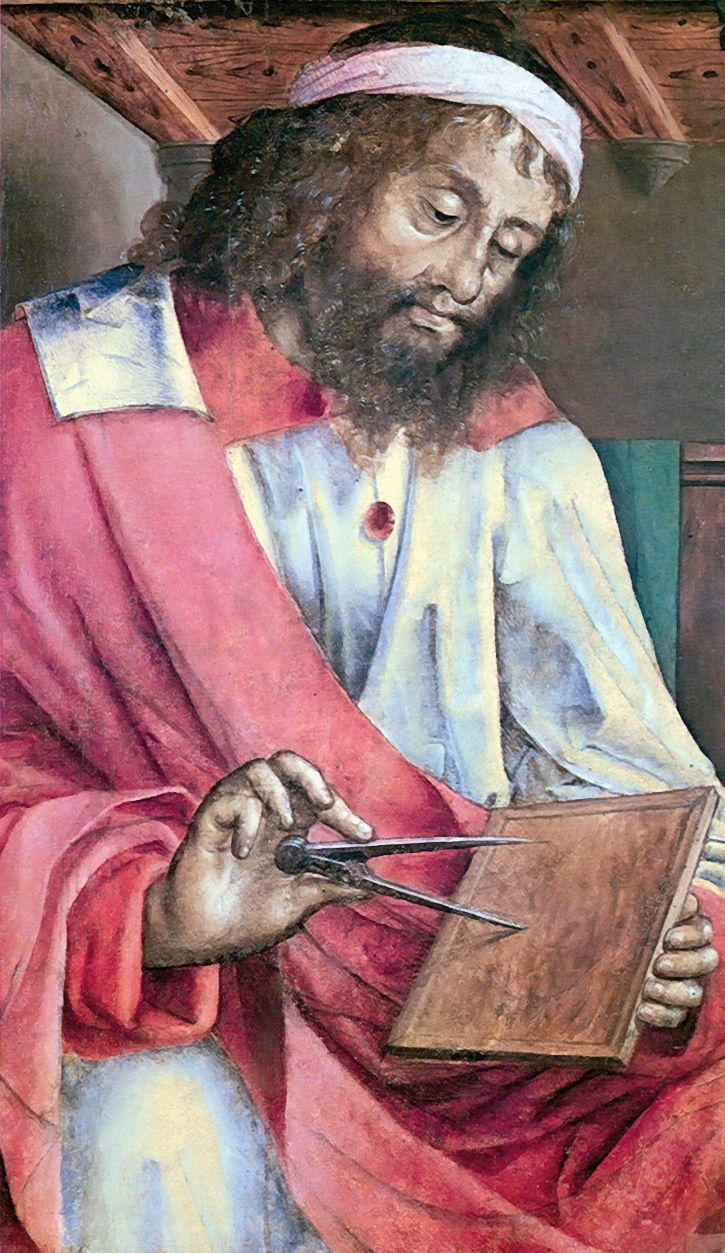
\includegraphics[width=\columnwidth]{media/Euklid.jpg}
    \end{column}
  \end{columns}
\end{frame}

\begin{frame}{Light travels in straight lines}
  \footfullcite{BBC:Let there be Light (2006)}
    \includemedia[label=euclid-straight-lines,
      width=\linewidth,height=0.6\linewidth, % 16:9
      activate=pageopen,
      addresource=media/euclid-straight-lines.mp4,
      flashvars={
        source=media/euclid-straight-lines.mp4
        &loop=false             % loop video
        &scaleMode=letterbox   % preserve aspect ratio while scaling the video
      }
    ]{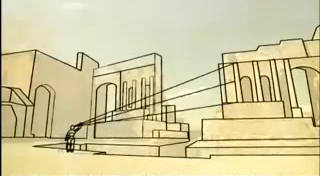
\includegraphics{media/euclid-straight-lines.png}}{VPlayer.swf}
\end{frame}

\begin{frame}{What is light?}
  Light is something that helps us see things. It travels in straight lines (well mostly!!).
\end{frame}

\section{Making a pinhole camera}
\frame{\tableofcontents[currentsection]}
\begin{frame}{Step 1}
  \begin{columns}
    \begin{column}{0.4\textwidth}
      Take a cup and scotch tape
    \end{column}
    \begin{column}{0.6\textwidth}
      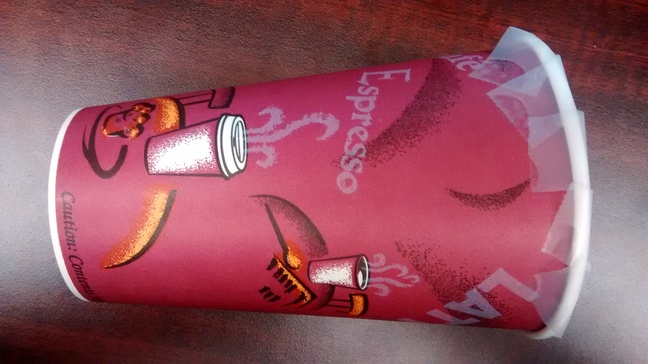
\includegraphics[width=\textwidth]{media/cup.jpg}\\
      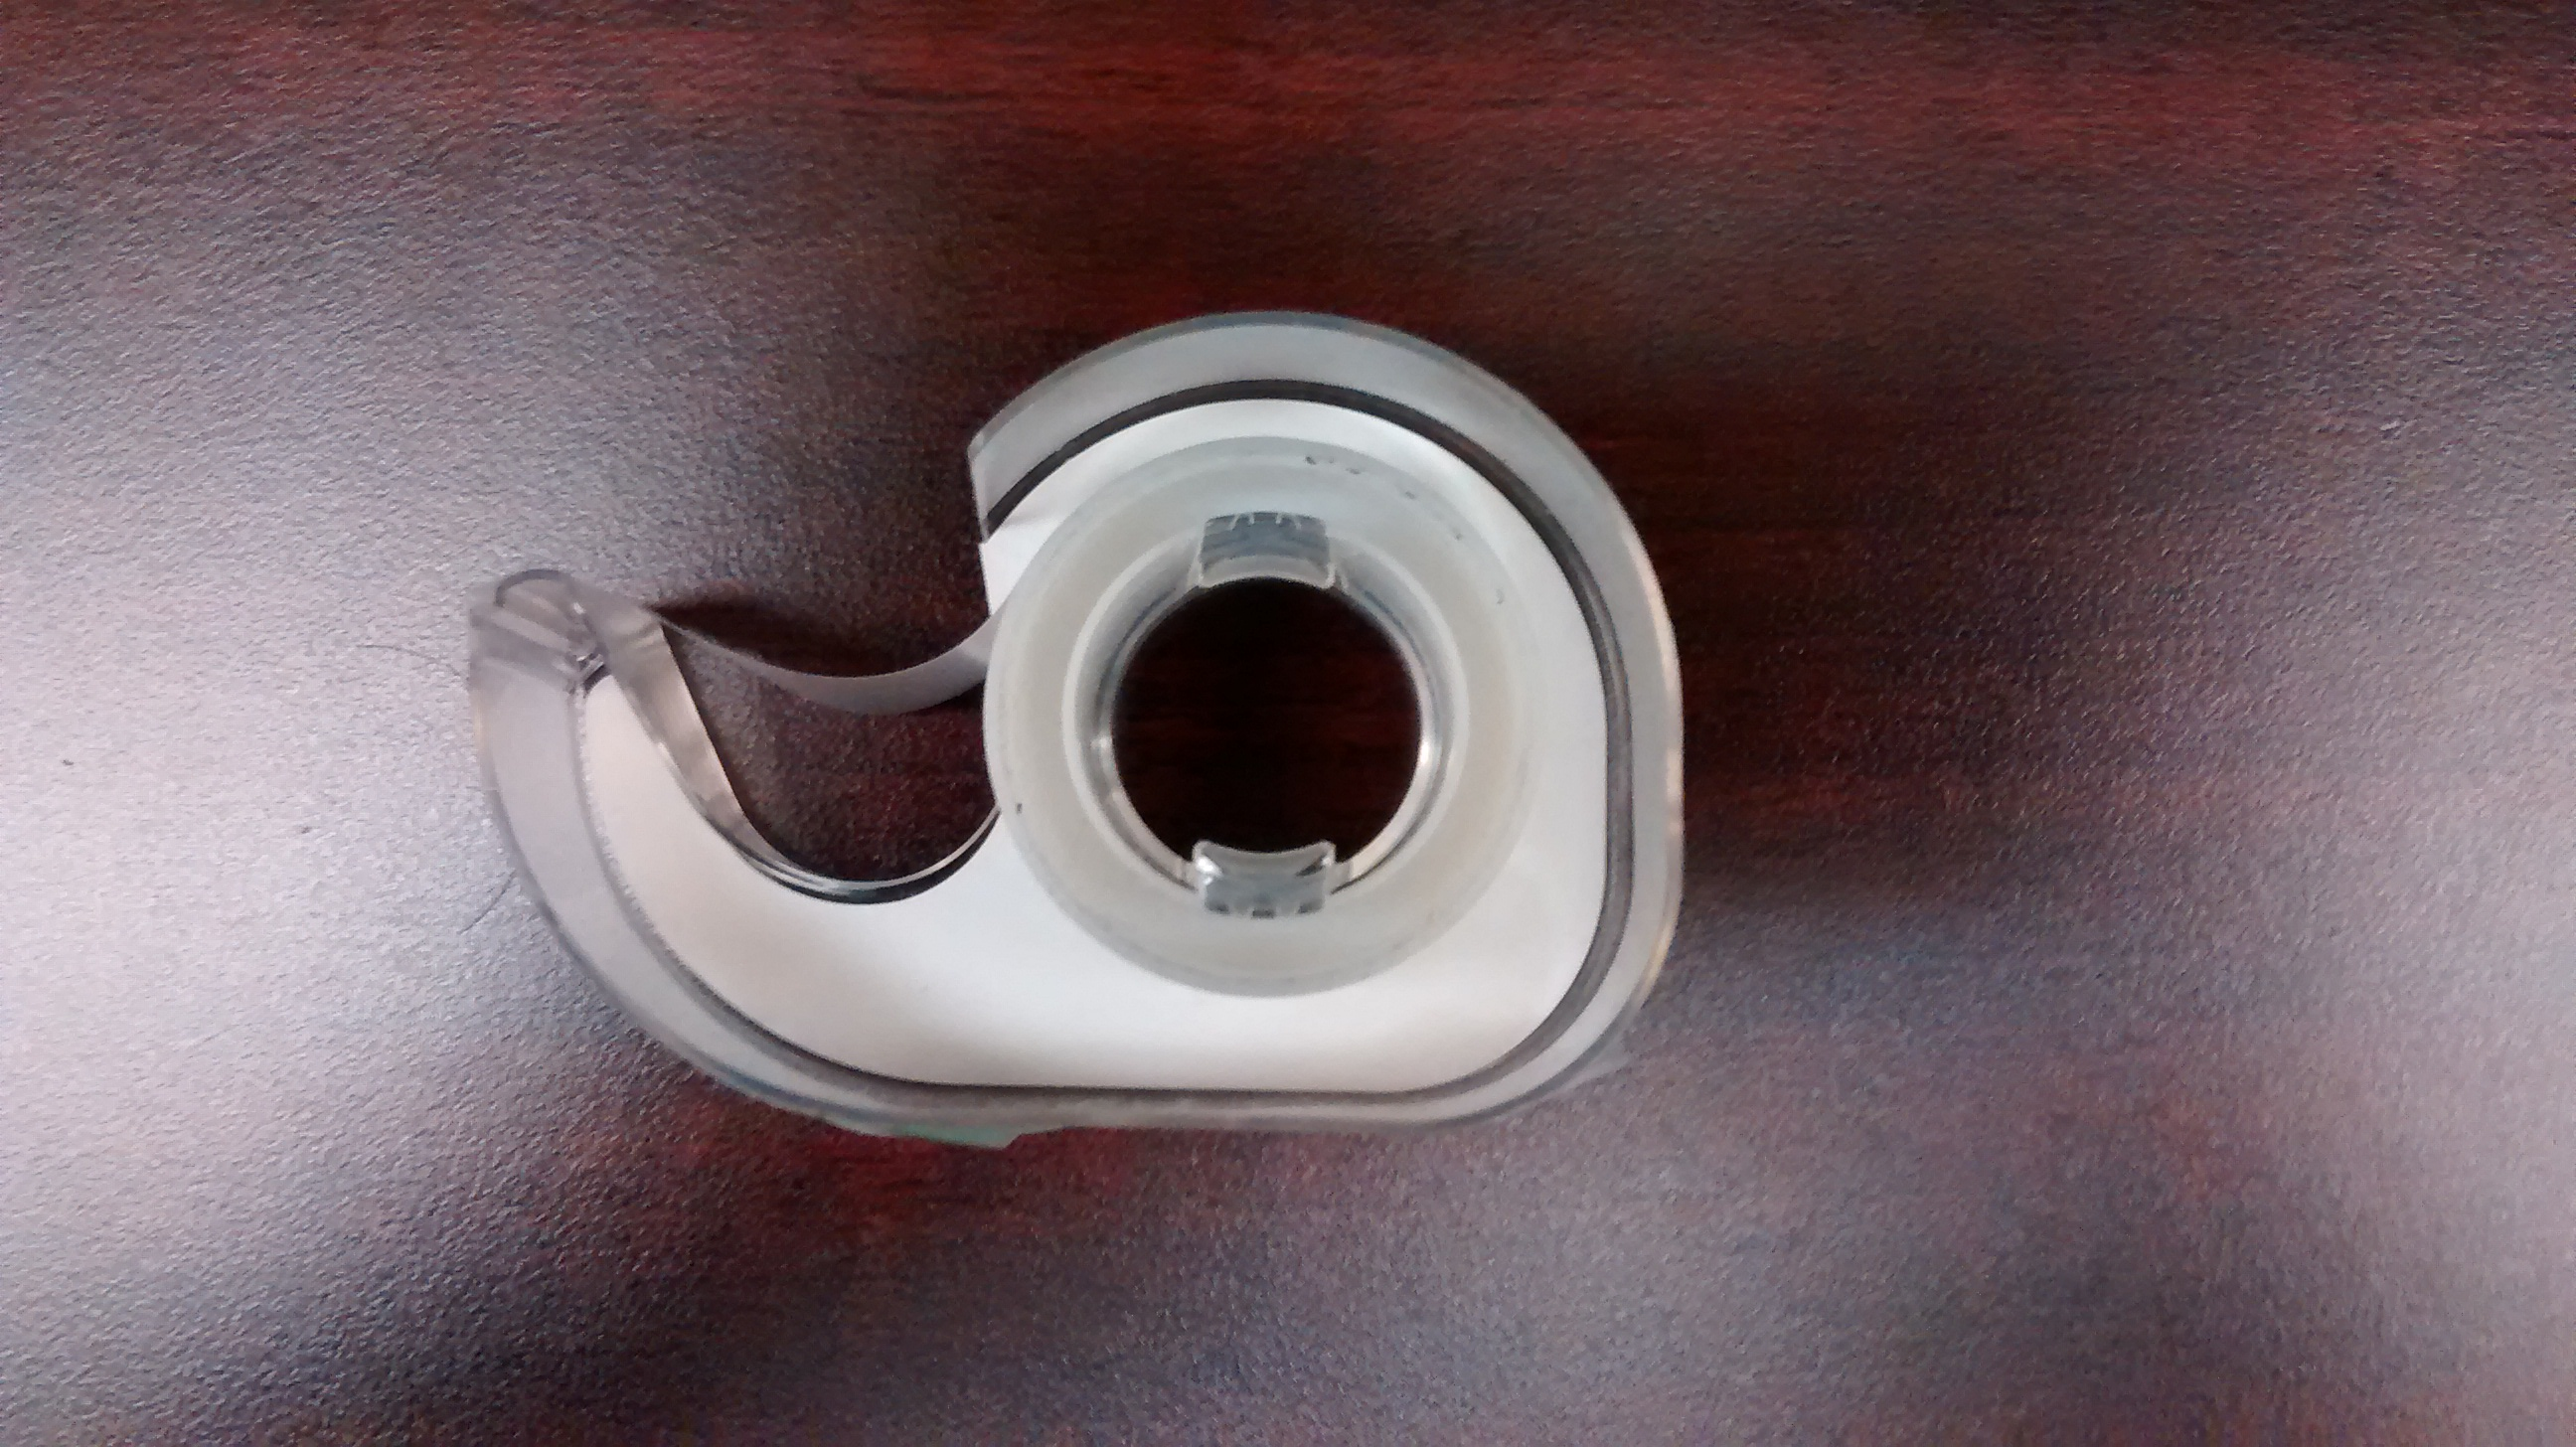
\includegraphics[width=\textwidth]{media/tape.jpg}
    \end{column}
  \end{columns}
\end{frame}

\begin{frame}{Step 2}
  \begin{columns}
    \begin{column}{0.6\textwidth}
      Cover the open end of cup using the scotch tape
    \end{column}
    \begin{column}{0.4\textwidth}
      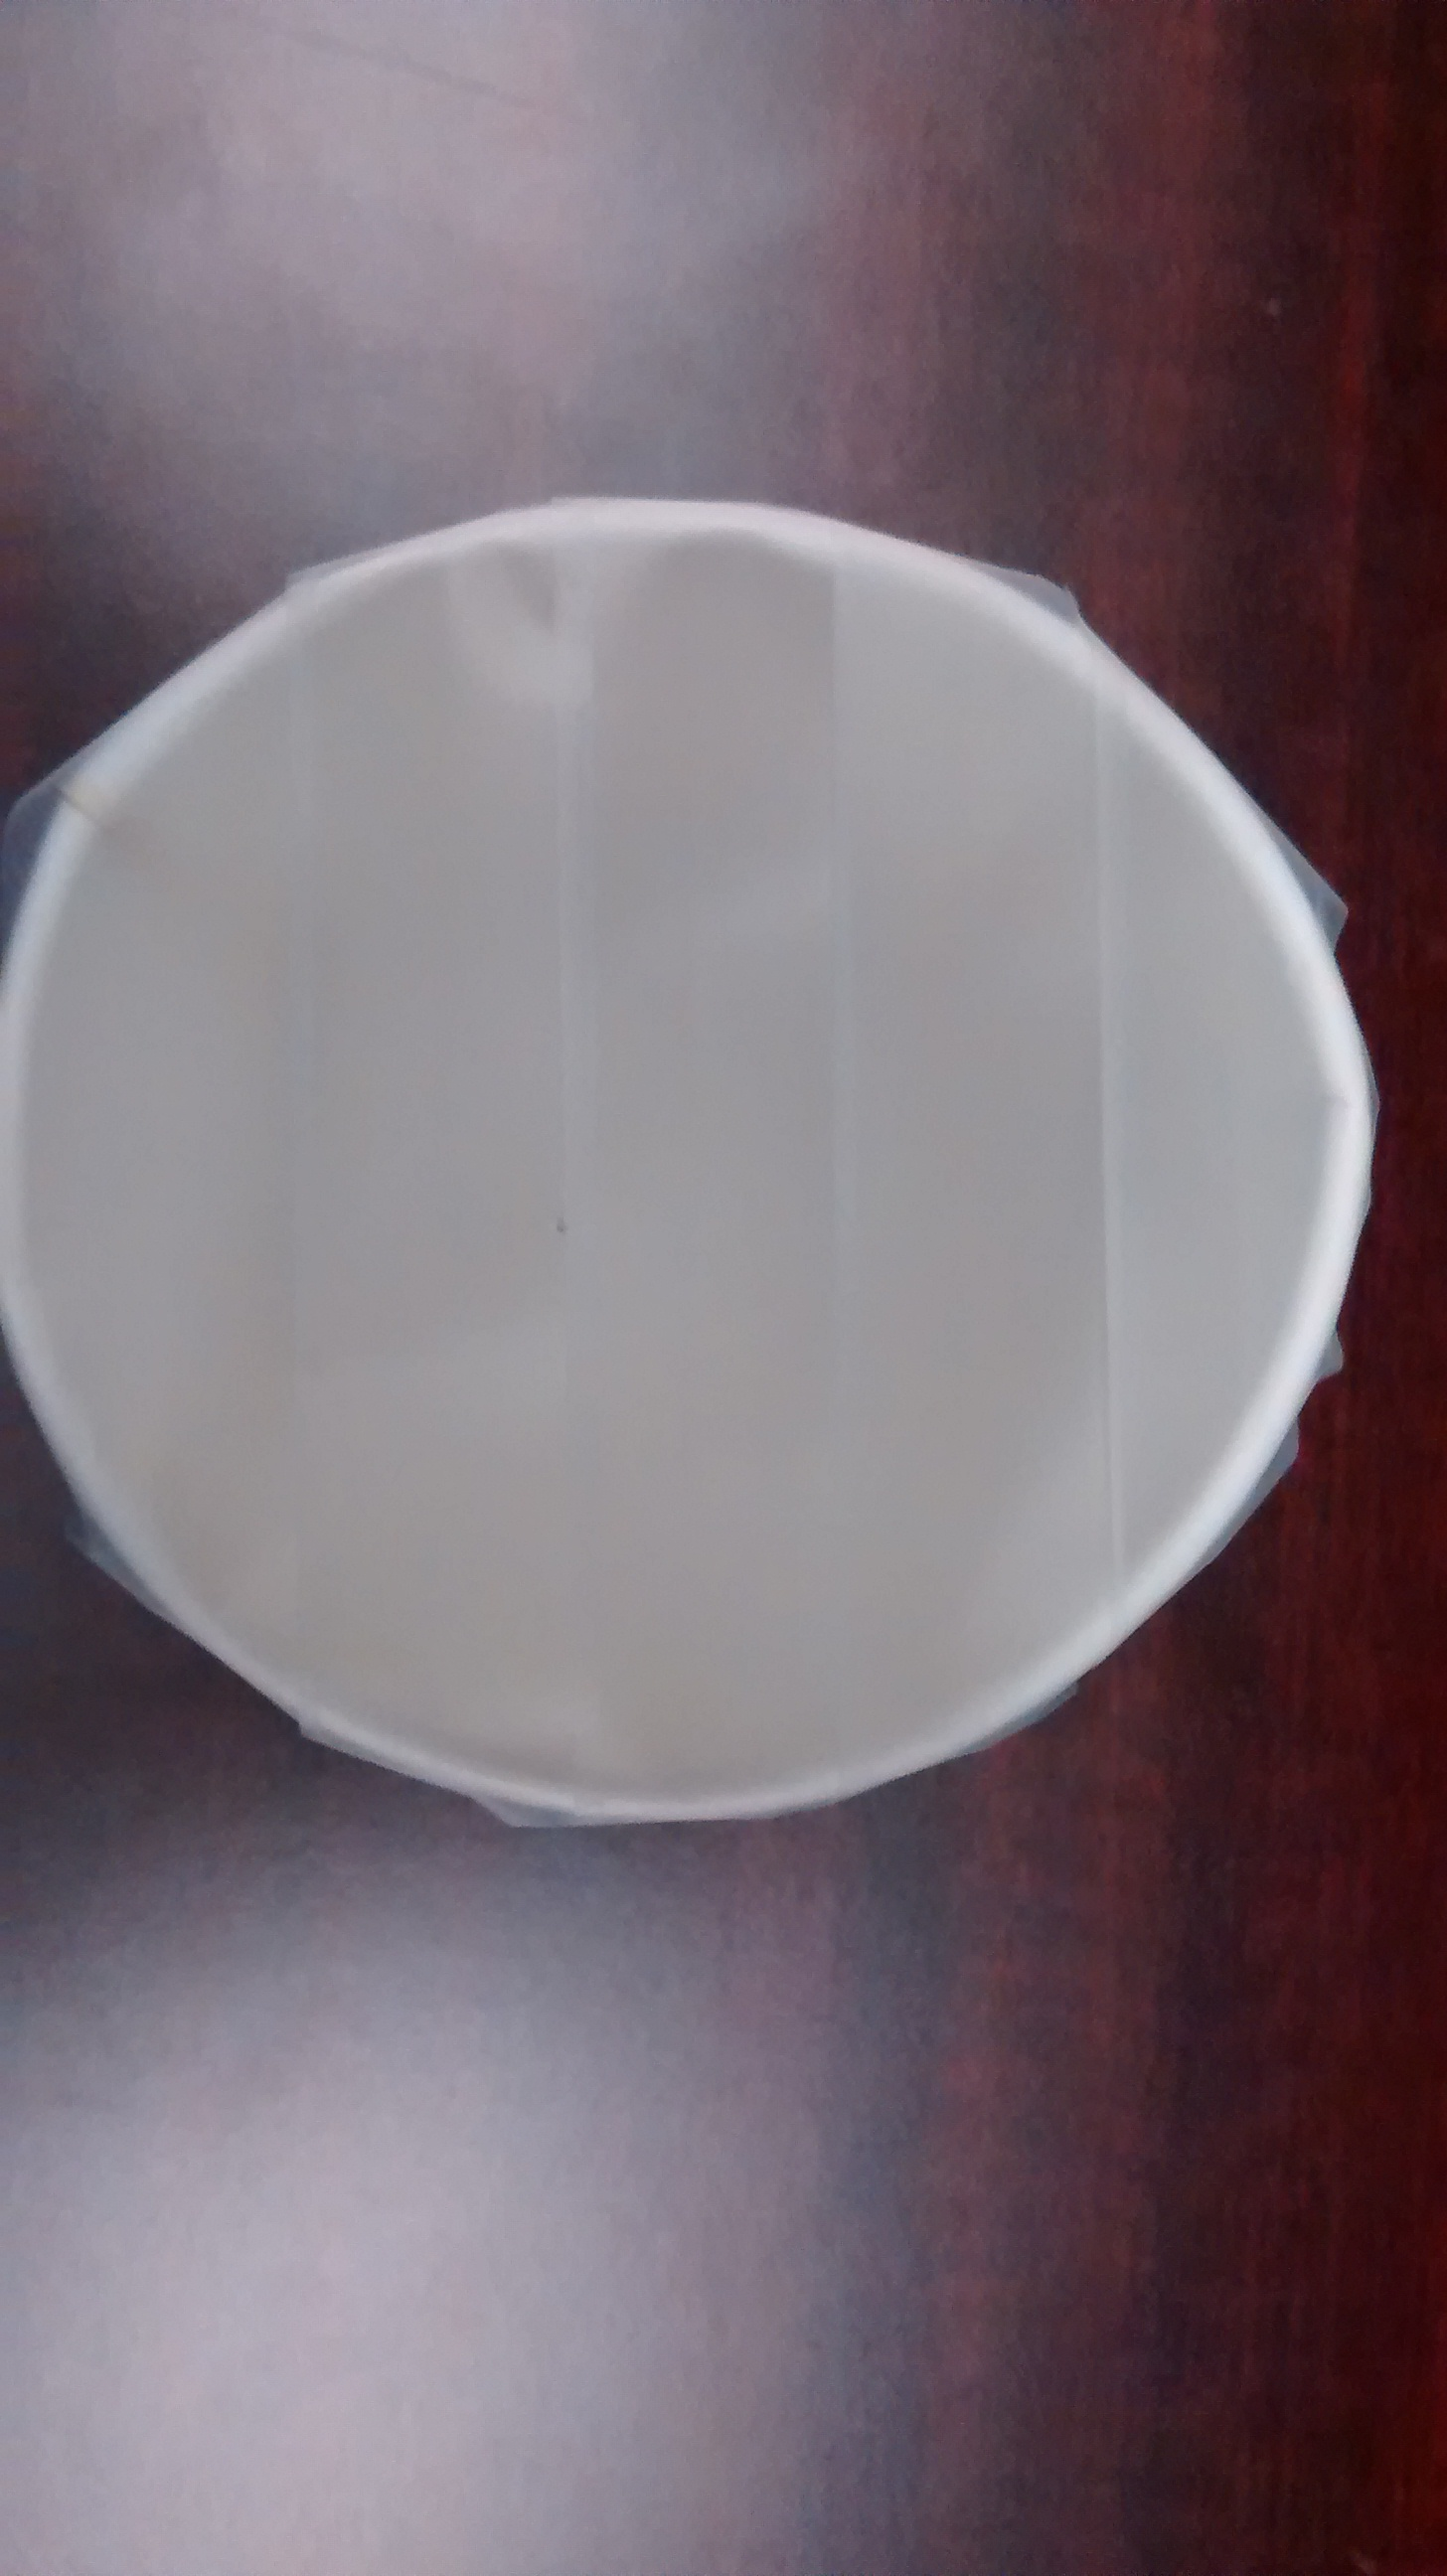
\includegraphics[width=\textwidth,trim=0 8in 0 4in,clip]{media/coveredlid2.jpg}\\
      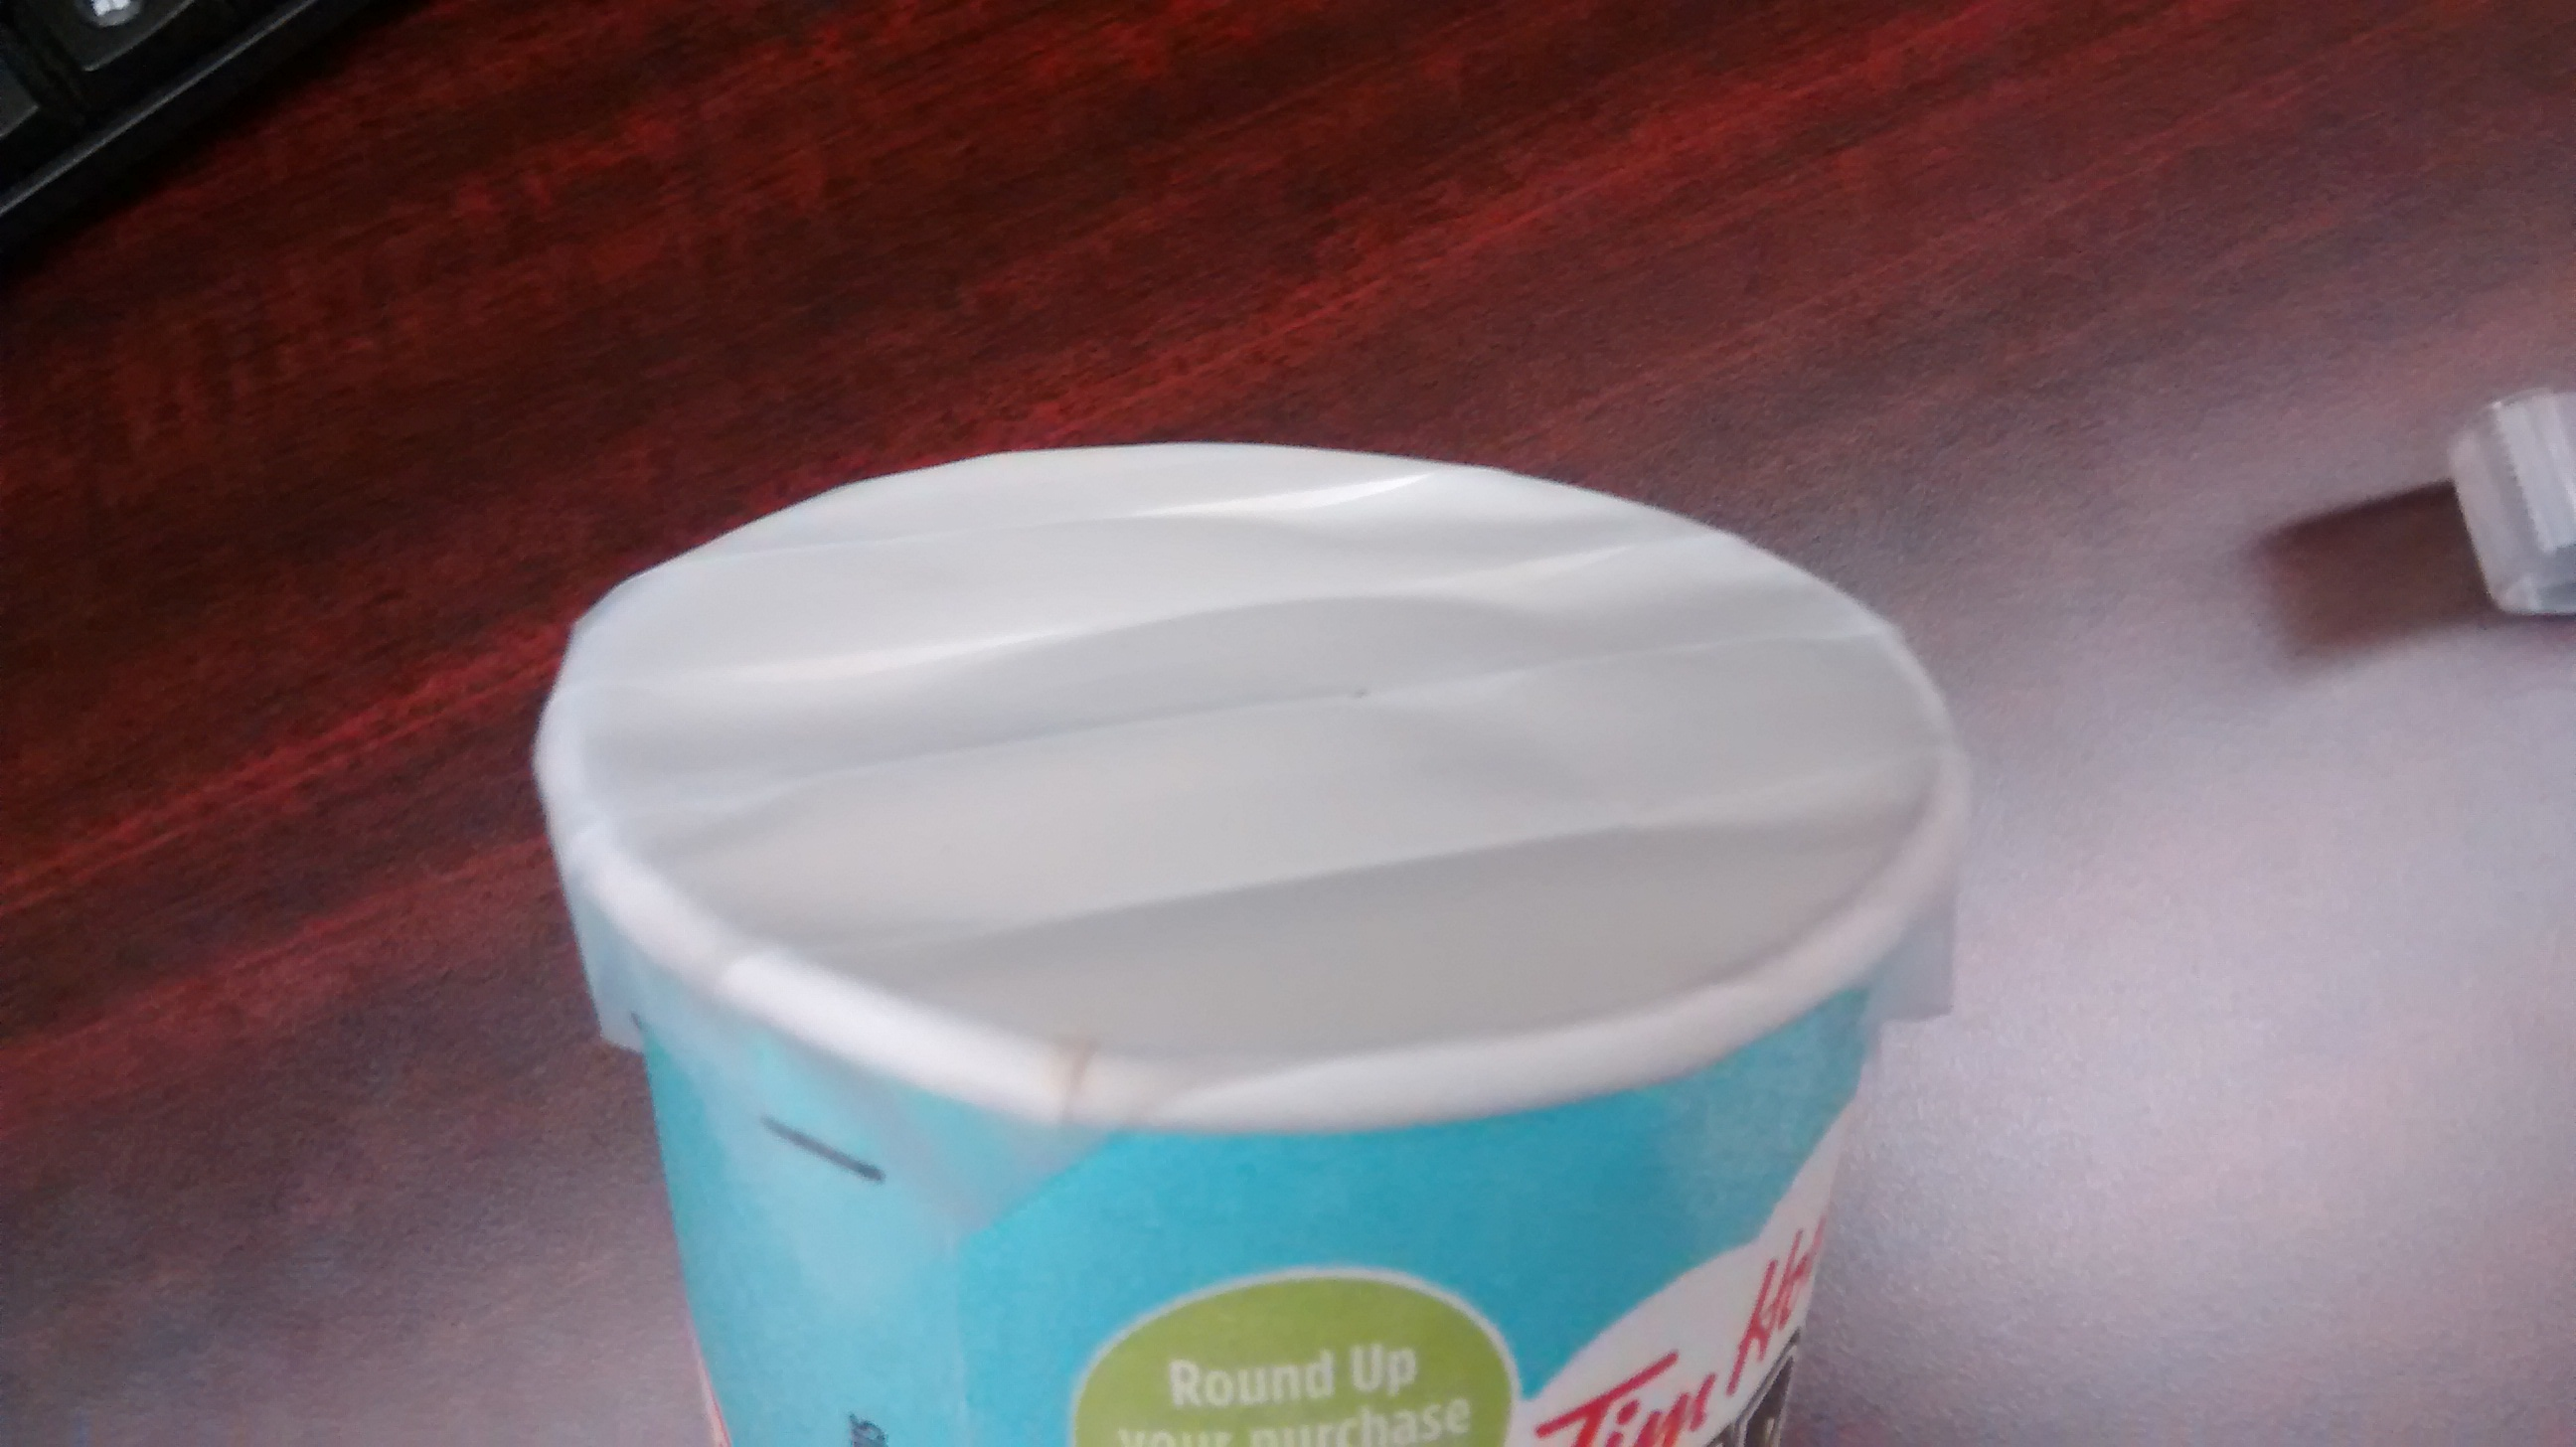
\includegraphics[width=\textwidth,trim=4in 0 4in 0,clip]{media/coveredlid1.jpg}
    \end{column}
  \end{columns}
\end{frame}

\begin{frame}{Step 3}
  \begin{columns}
    \begin{column}{0.6\textwidth}
      Cut a circular piece of construction paper to reinforce the cup base.
    \end{column}
    \begin{column}{0.4\textwidth}
      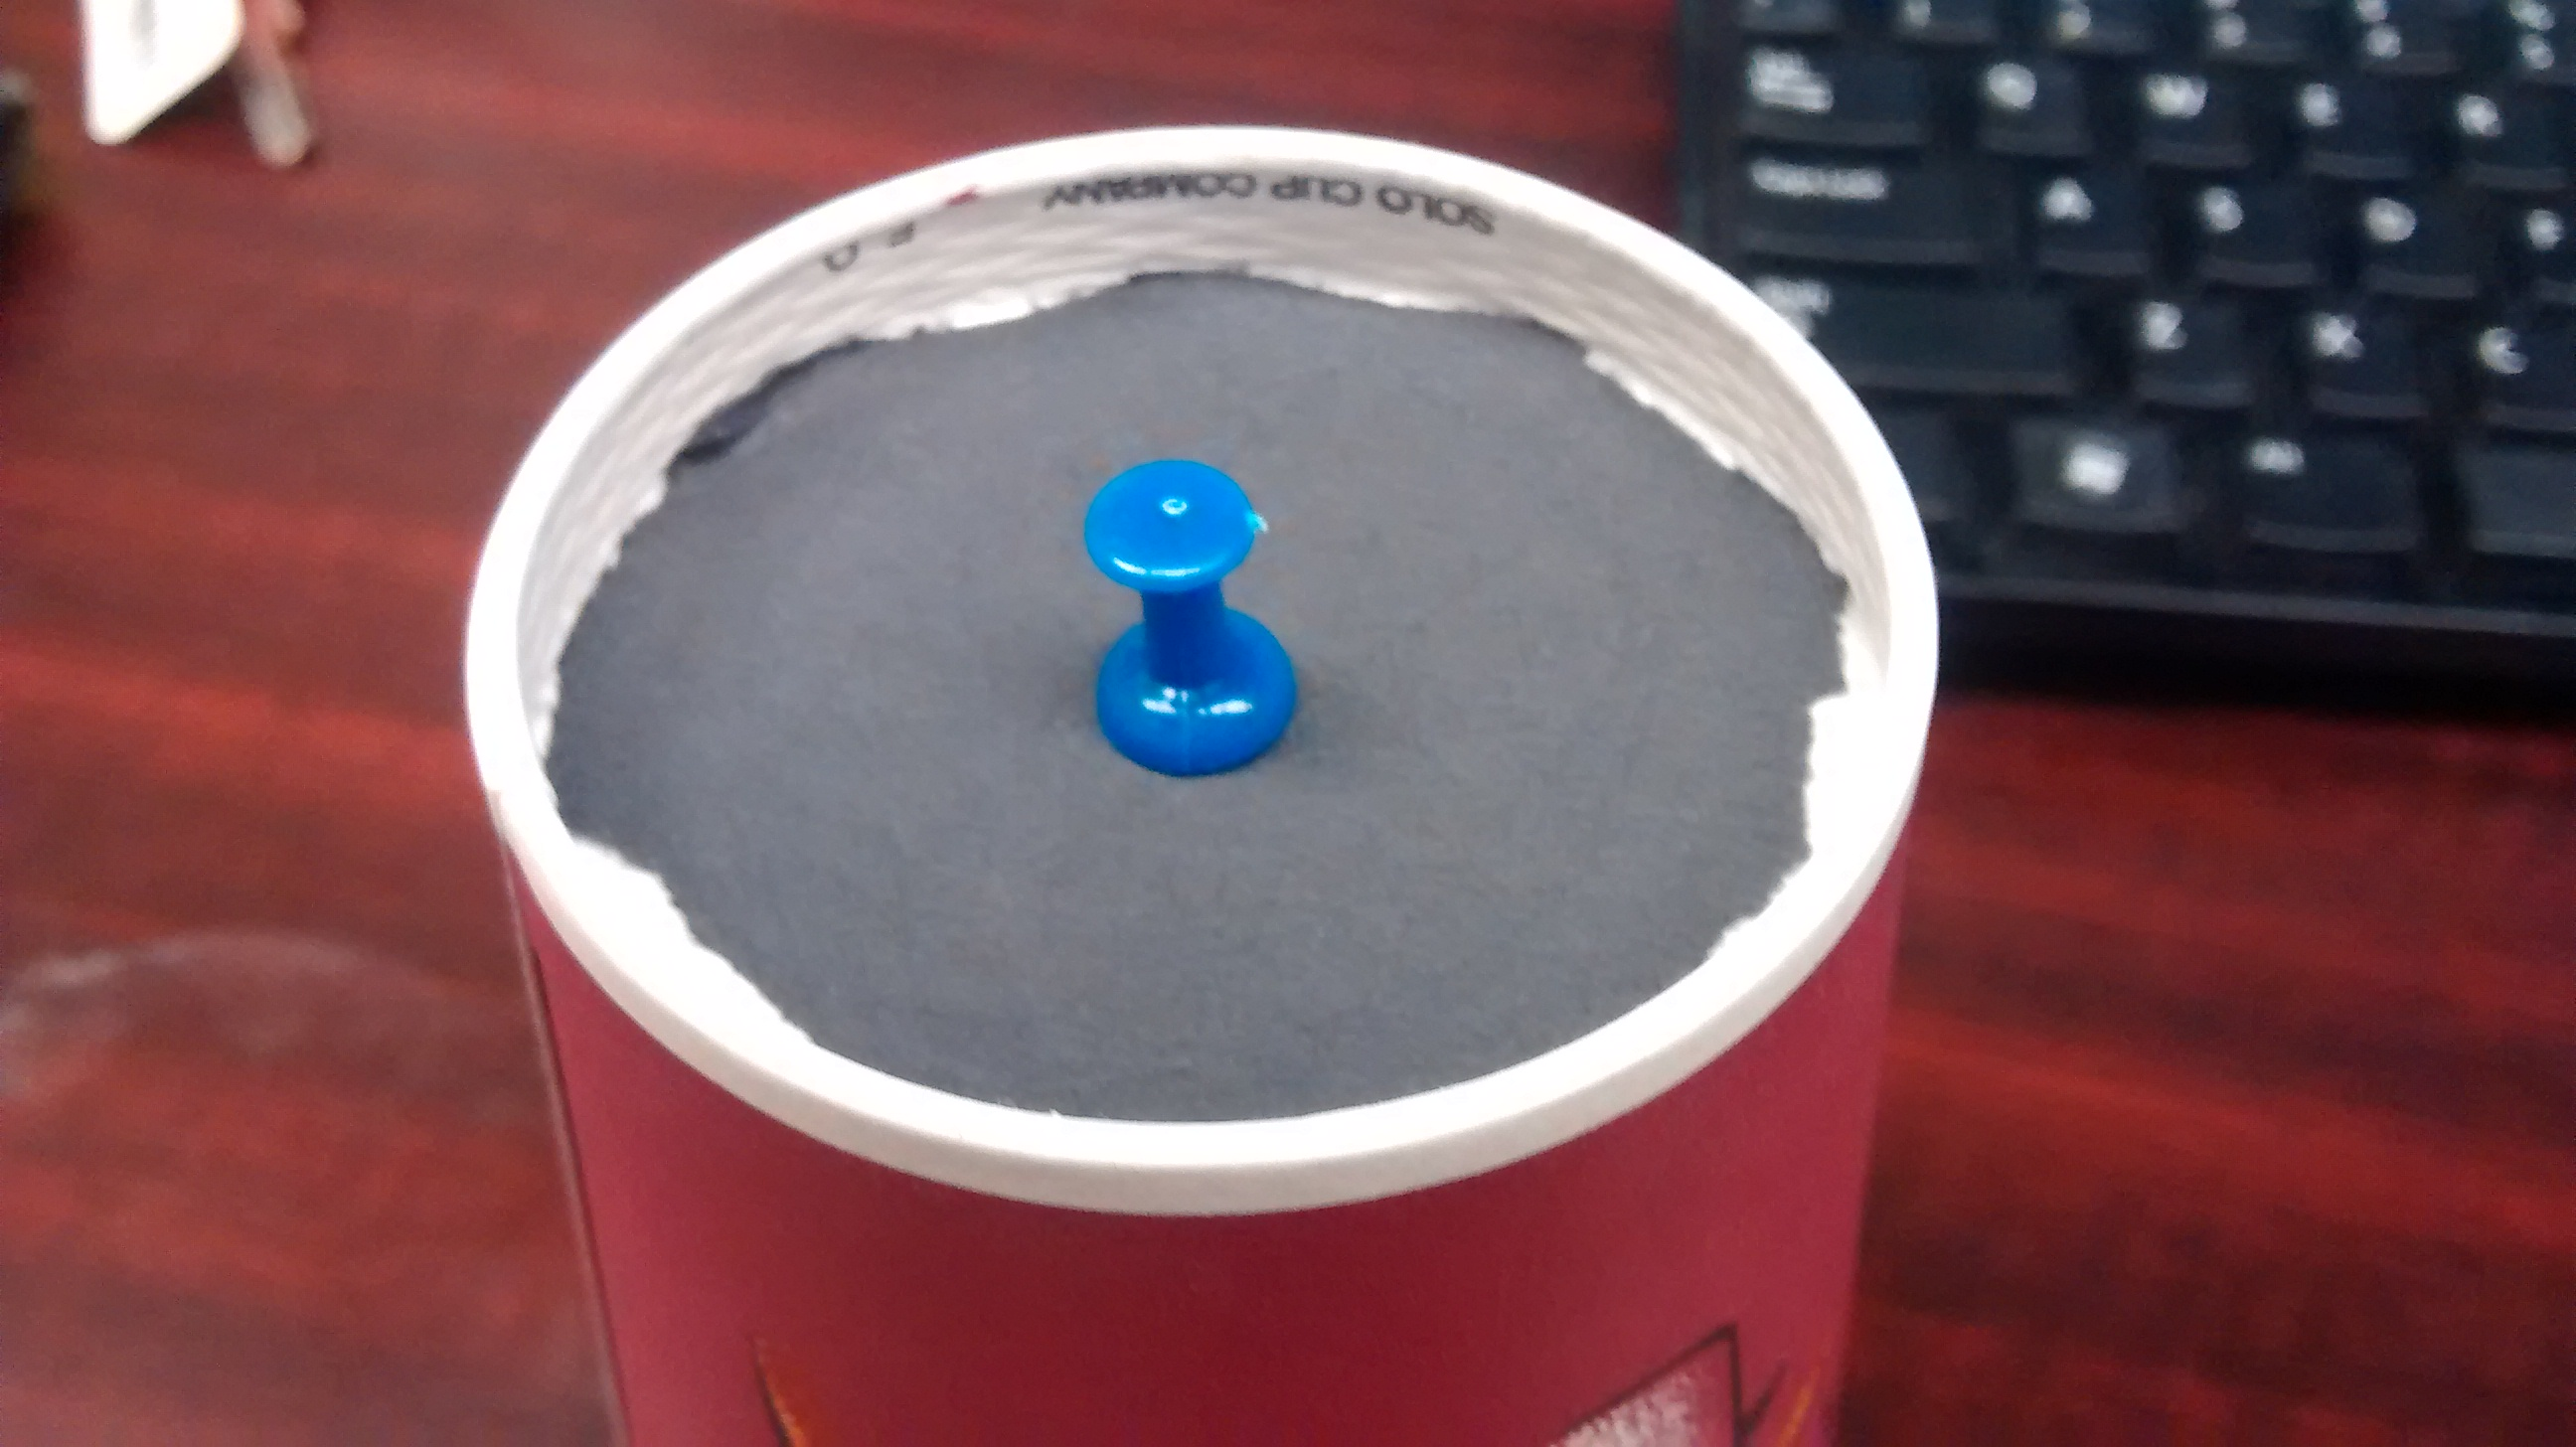
\includegraphics[width=\textwidth]{media/pushpin.jpg}
    \end{column}
  \end{columns}
  
\end{frame}

\begin{frame}{Step 4}
  \begin{columns}
    \begin{column}{0.6\textwidth}
      Pierce a pinhole through the closed end of the cup using a push pin
    \end{column}
    \begin{column}{0.4\textwidth}
      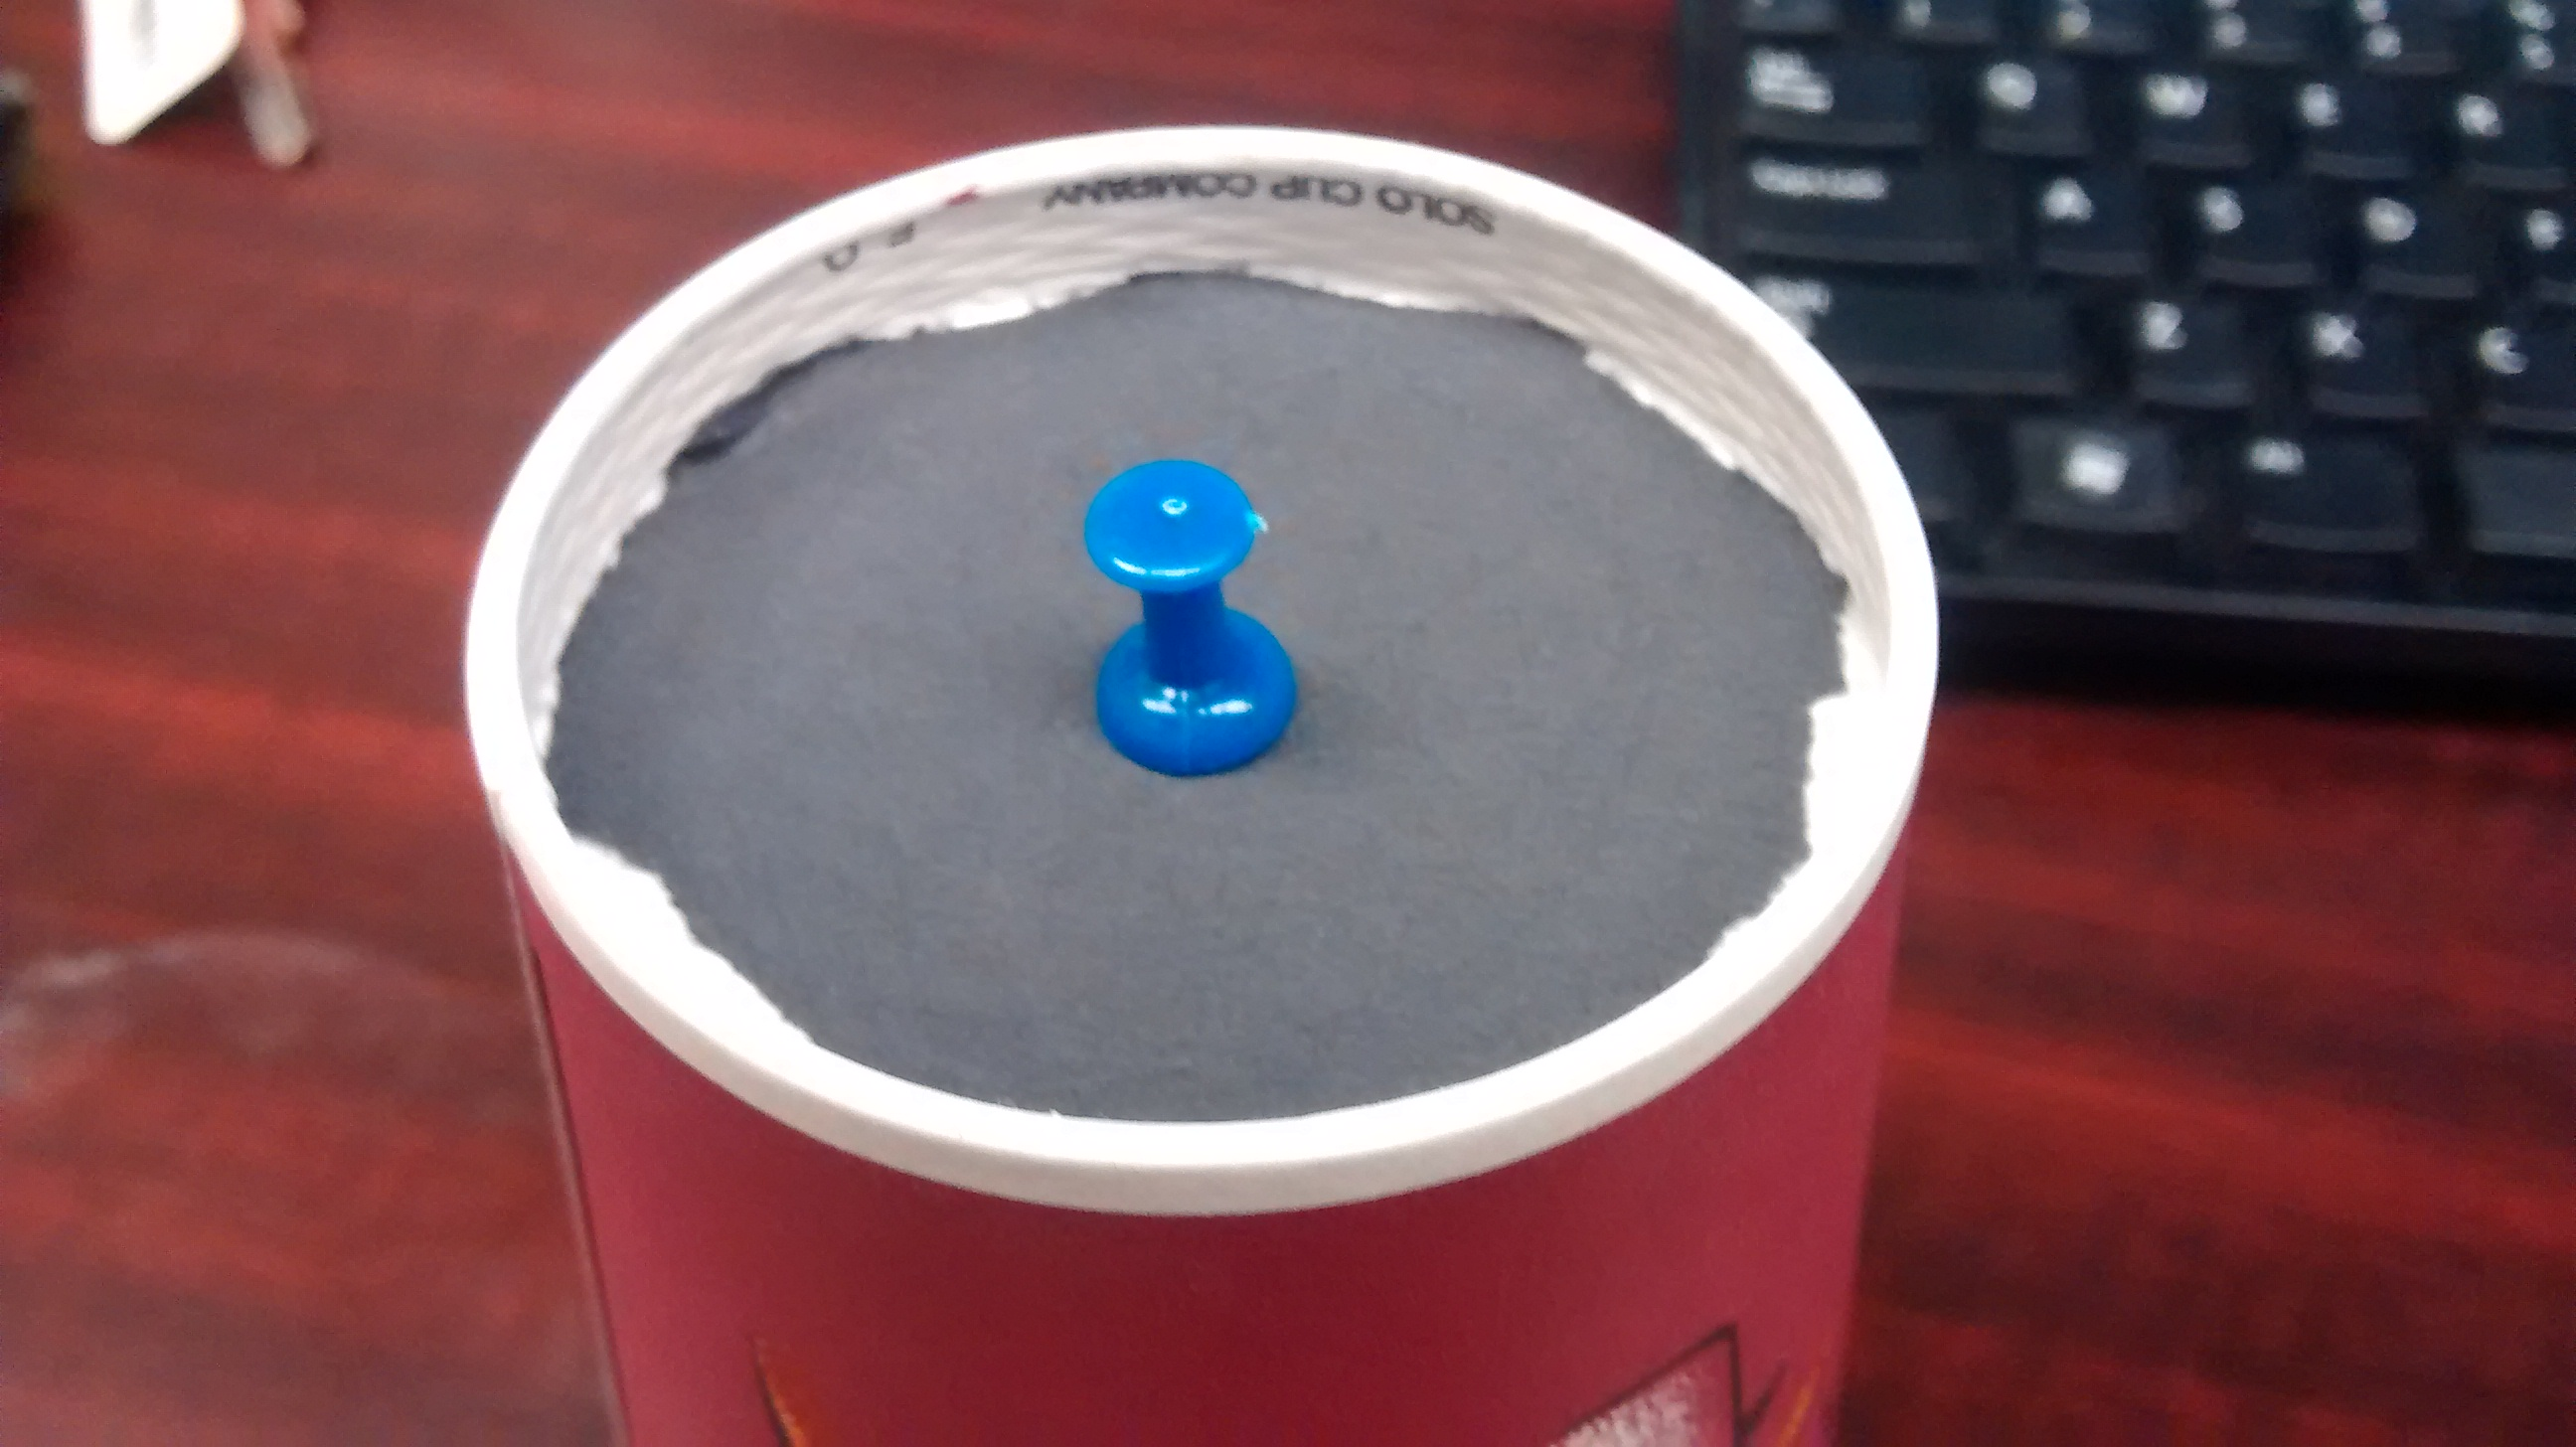
\includegraphics[width=\textwidth]{media/pushpin.jpg}
    \end{column}
  \end{columns}
\end{frame}

\begin{frame}[fragile]{Scientific method}
  
             \newcommand{\textonecolor}[1]{\ifnum2<#1black\else black!50\fi}
  \only<2>{\renewcommand{\textonecolor}[1]{\ifnum3<##1black\else black!50\fi}}
  \only<4>{\renewcommand{\textonecolor}[1]{\ifnum4<##1black\else black!50\fi}}

             \newcommand{\nodeonecolor}[1]{\if3#1red!20\else none\fi}
  \only<2>{\renewcommand{\nodeonecolor}[1]{\if4##1red!20\else none\fi}}
  \only<4>{\renewcommand{\nodeonecolor}[1]{\if5##1red!20\else none\fi}}
  \begin{center}
    \begin{tikzpicture}[]

      \def \n {6}
      \def \radius {3}
      \def \margin {15} % margin in angles, depends on the radius

      \foreach \s/\t in {1/Purpose,2/Research,3/Hypothesis,4/Experiment,5/Analysis,6/Conclusion}
      {
        \node[fill=\nodeonecolor{\s},text=\textonecolor{\s},circle,minimum width=3] at ({360/\n * (\s - 1)}:\radius) {\t};
        \draw[->, >=latex] ({360/\n * (\s - 1)+\margin}:\radius) 
        arc ({360/\n * (\s - 1)+\margin}:{360/\n * (\s)-\margin}:\radius);
      }
    \end{tikzpicture}
    \addtooverlay<.(3)>{%
      \draw[fill=black,opacity=1.00] 
      (current page.north east) rectangle (current page.south west);
      \node at (current page.center) {
\includegraphics[height=\textheight]{media/tree.png}};
    }
  \end{center}

\end{frame}

\begin{frame}{Did you see an inverted image?}
  \centering
  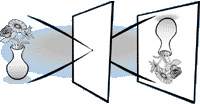
\includegraphics{media/upside_down_vase.png}
\end{frame}

\section{How does it work}
\begin{frame}{Ray diagram}
  \begin{tikzpicture}[scale=0.8]
    \node [anchor=south west] (img) at (0,0) {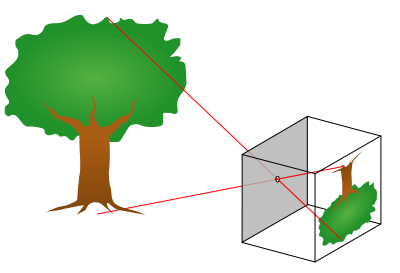
\includegraphics[width=0.8\textwidth]{media/pinhole.png}};
    \begin{scope}[x={(img.south east)},y={(img.north west)}]
      \fill [yellow] (0.75,1.2) node (sun) {} ellipse (0.06 and 0.08);
\coordinate (tree) at (0.2,0.7);
      \foreach \y in {10, 20, 30} 
      {
        \draw [very thick,yellow] ($(sun) + (-150+\y:.1)$) -- ($(tree) + (80-2*\y:.3)$) node [inner sep=0] (trays) {};
	}
    \end{scope}
  \end{tikzpicture}
\end{frame}

\begin{frame}{Camera Obscura: Camera in a room}
    \includemedia[label=camera-ina-room,
      width=\linewidth,height=0.6\linewidth, % 16:9
      activate=pageopen,
      addresource=media/camera_ina_room.mp4,
      flashvars={
        source=media/camera_ina_room.mp4
        &loop=false             % loop video
        &scaleMode=letterbox   % preserve aspect ratio while scaling the video
      }
    ]{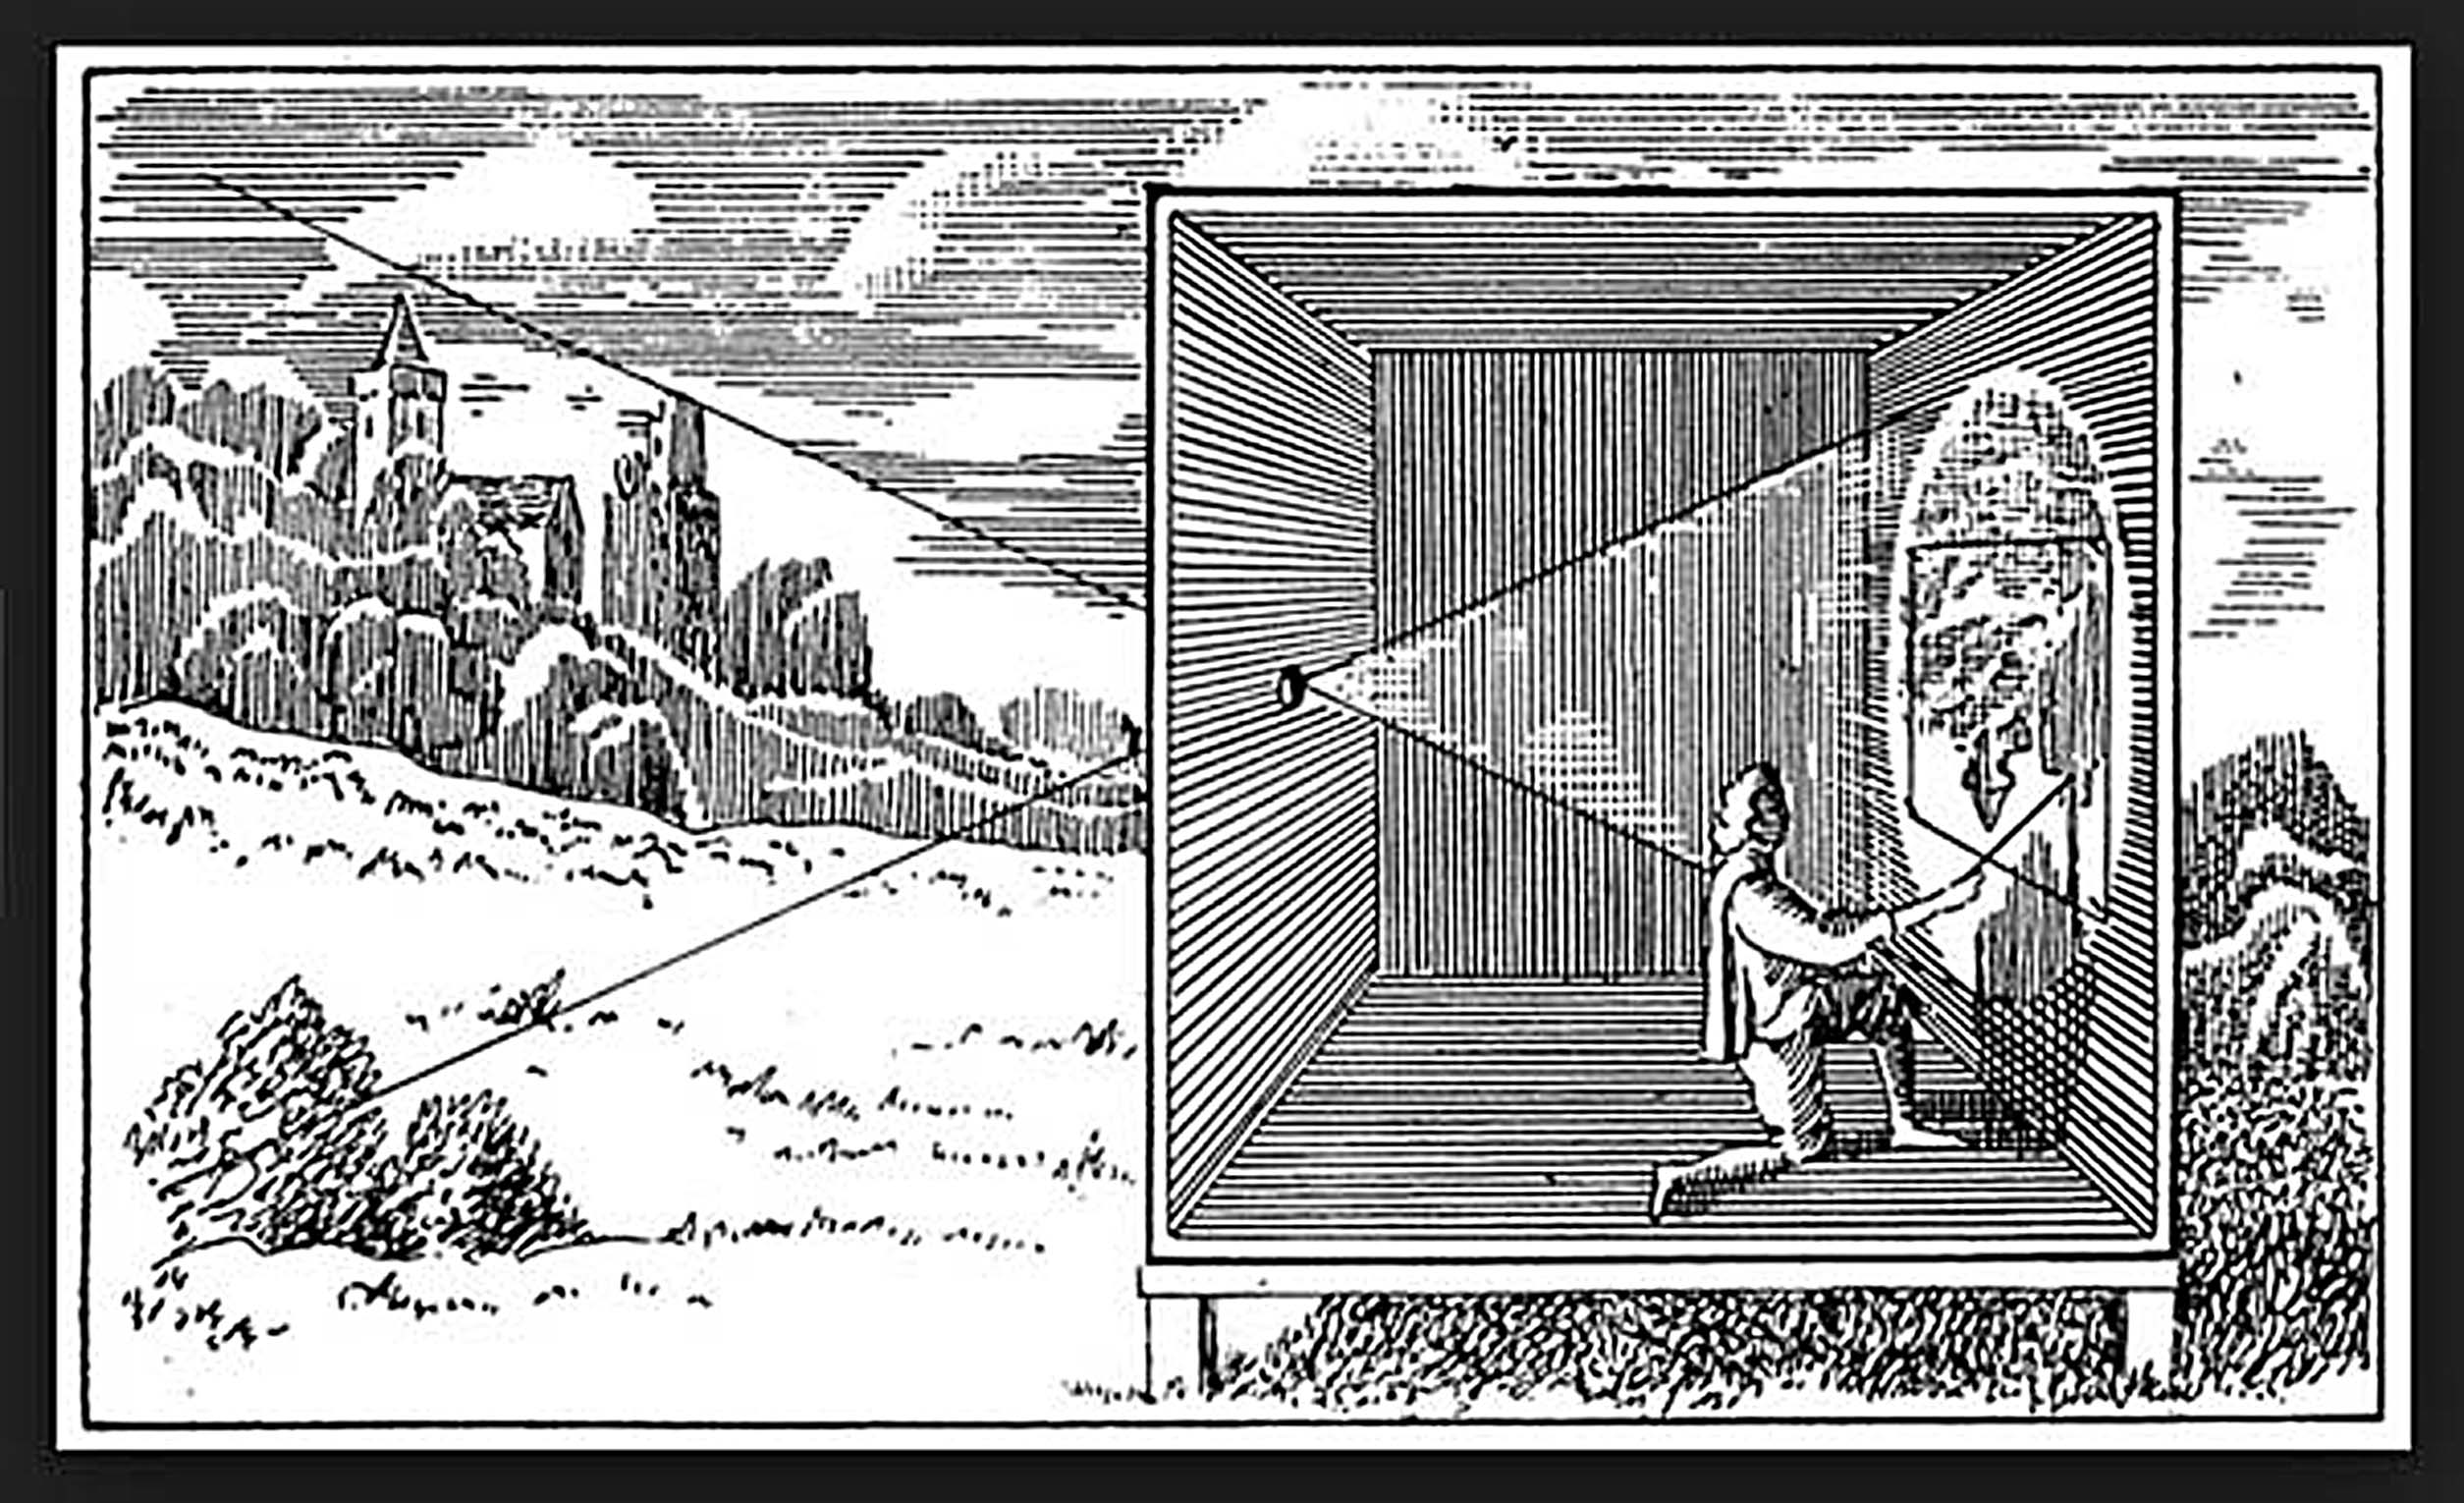
\includegraphics{media/camera_ina_room.jpg}}{VPlayer.swf}
\end{frame}

\begin{frame}{Camera Obscura: Camera in a room}
  \centering
  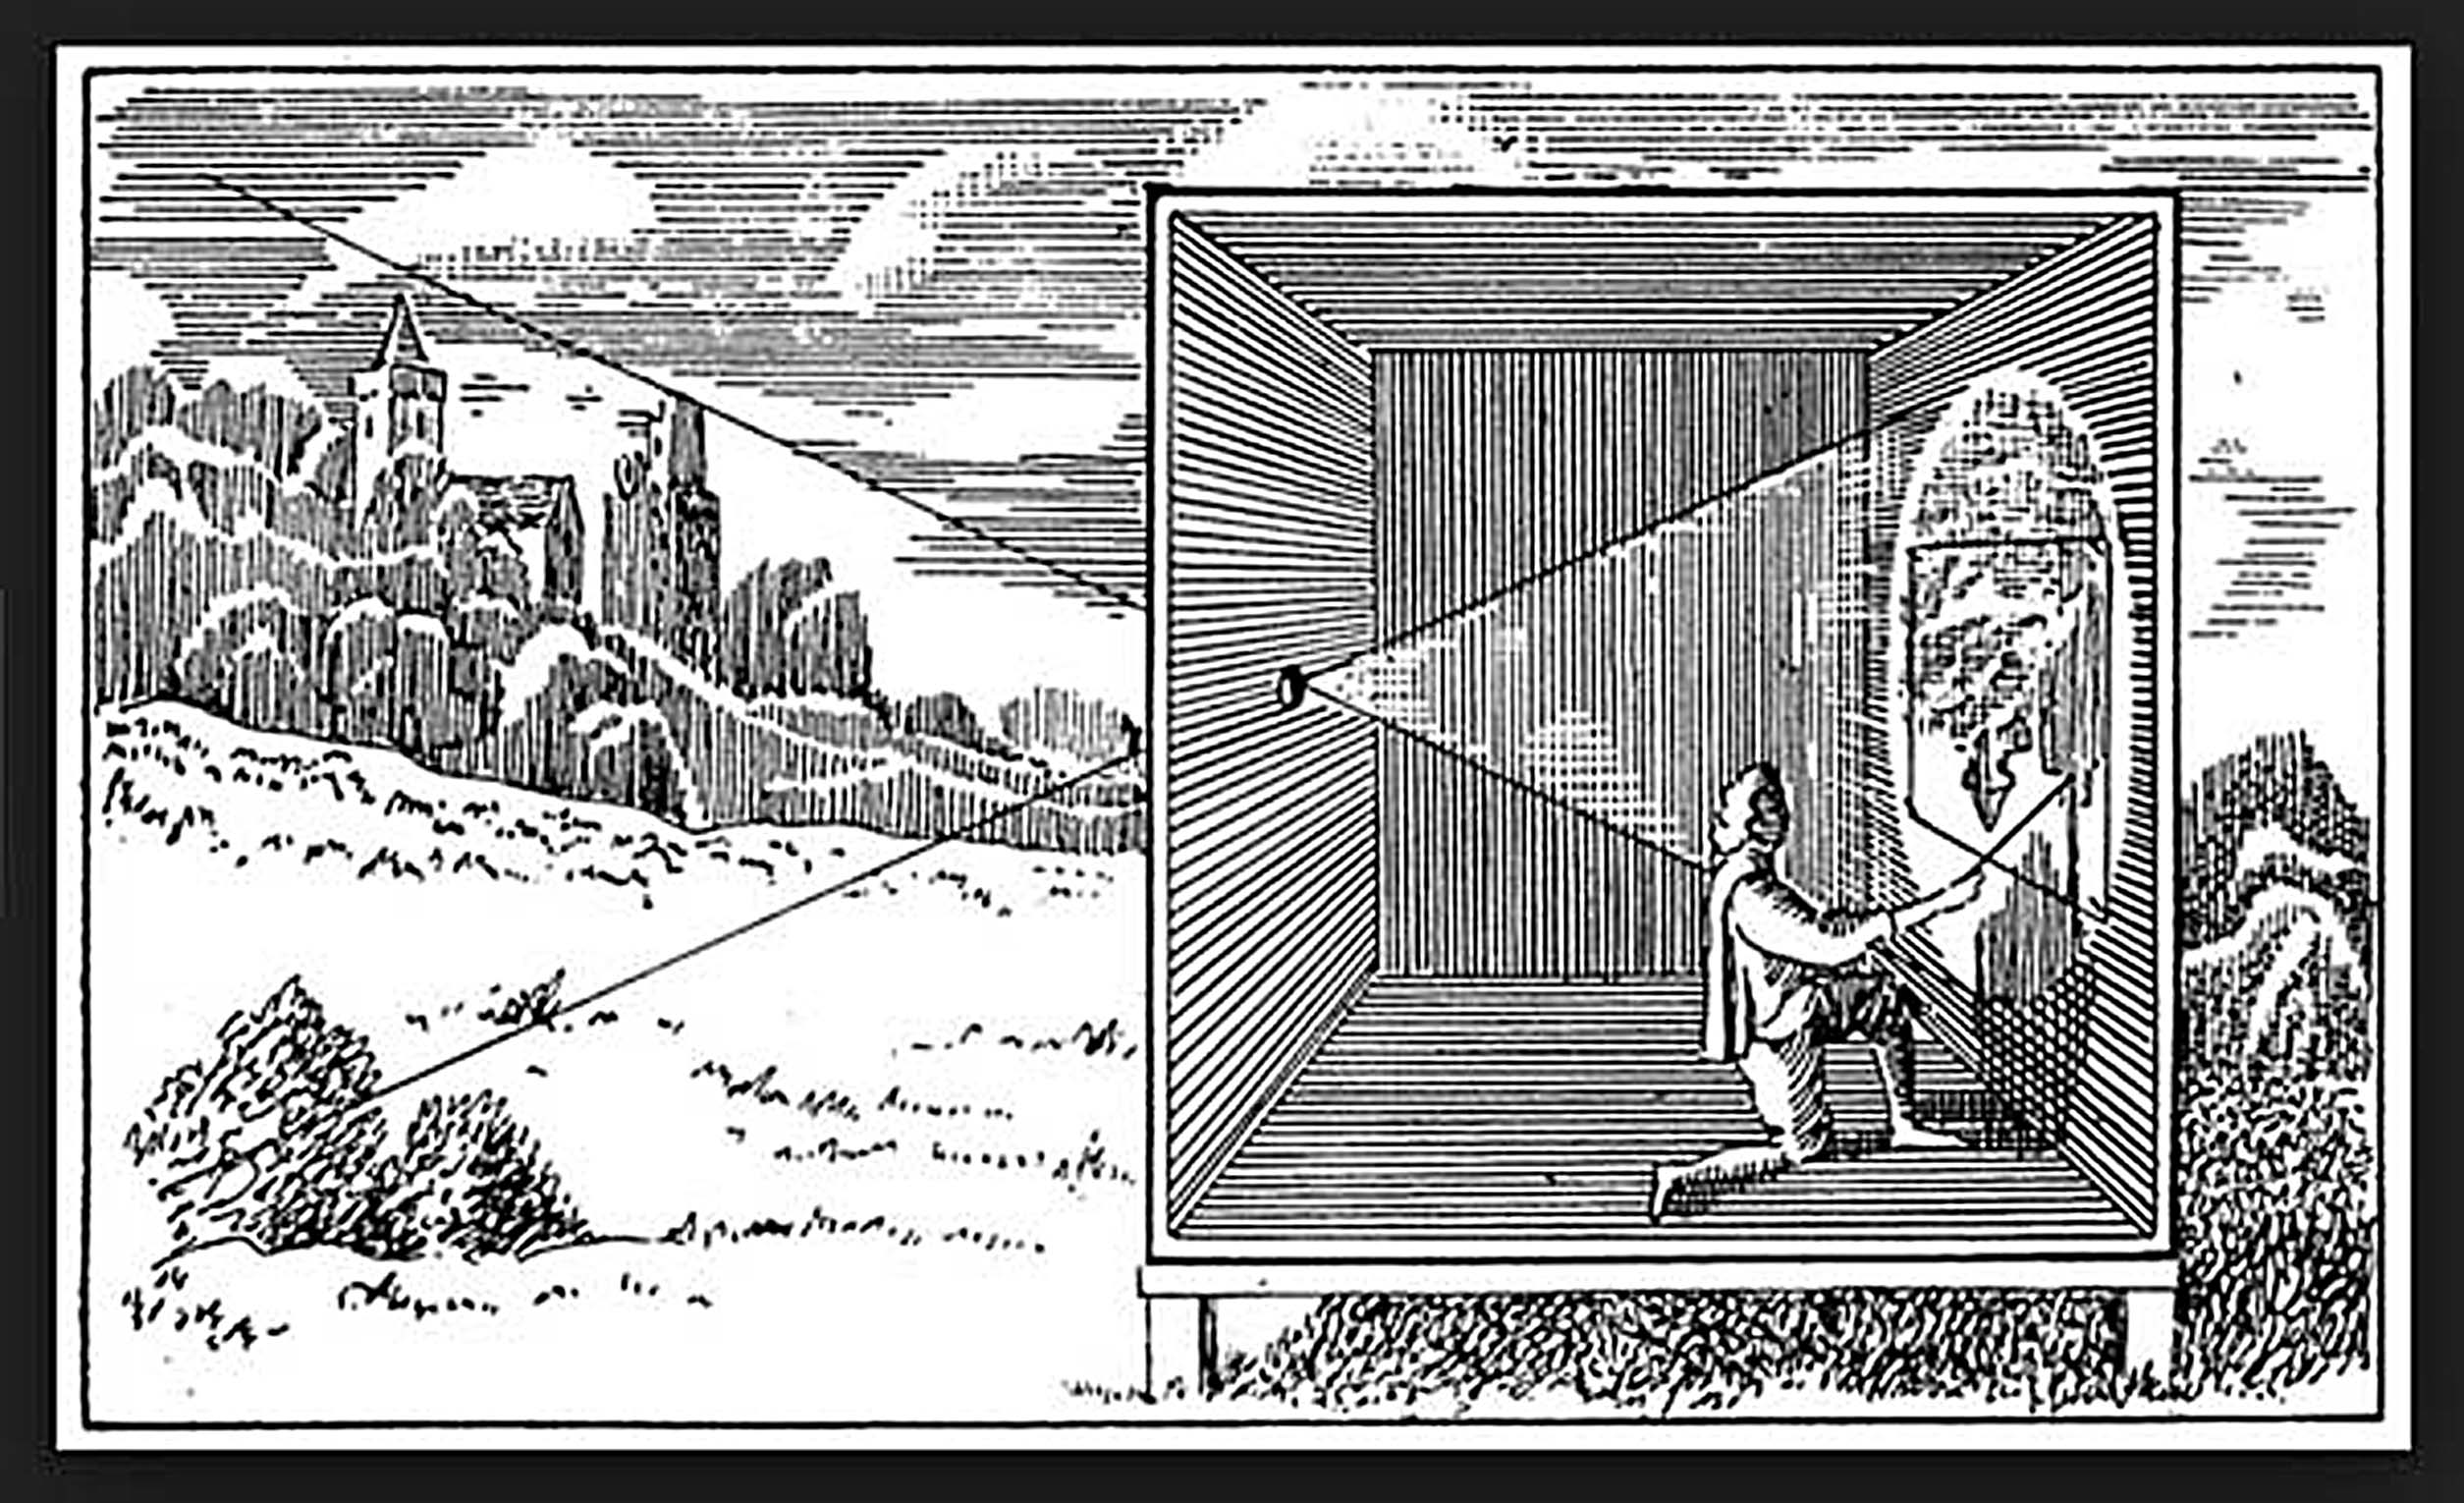
\includegraphics[width=\textwidth]{media/camera_ina_room.jpg}
\end{frame}

\section{Effect of distance}
\begin{frame}{Guess what happens}
  ... if you change the distance of the pinhole from the object?
\end{frame}

\begin{frame}[fragile]{Scientific method}
  
             \newcommand{\textonecolor}[1]{\ifnum2<#1black\else black!50\fi}
  \only<2>{\renewcommand{\textonecolor}[1]{\ifnum3<##1black\else black!50\fi}}
  \only<4>{\renewcommand{\textonecolor}[1]{\ifnum4<##1black\else black!50\fi}}

             \newcommand{\nodeonecolor}[1]{\if3#1red!20\else none\fi}
  \only<2>{\renewcommand{\nodeonecolor}[1]{\if4##1red!20\else none\fi}}
  \only<4>{\renewcommand{\nodeonecolor}[1]{\if5##1red!20\else none\fi}}
  \begin{center}
    \begin{tikzpicture}[]

      \def \n {6}
      \def \radius {3}
      \def \margin {15} % margin in angles, depends on the radius

      \foreach \s/\t in {1/Purpose,2/Research,3/Hypothesis,4/Experiment,5/Analysis,6/Conclusion}
      {
        \node[fill=\nodeonecolor{\s},text=\textonecolor{\s},circle,minimum width=3] at ({360/\n * (\s - 1)}:\radius) {\t};
        \draw[->, >=latex] ({360/\n * (\s - 1)+\margin}:\radius) 
        arc ({360/\n * (\s - 1)+\margin}:{360/\n * (\s)-\margin}:\radius);
      }
    \end{tikzpicture}
    \addtooverlay<.(3)>{%
      \draw[fill=black,opacity=1.00] 
      (current page.north east) rectangle (current page.south west);
      \node at (current page.center) {
\includegraphics[height=\textheight]{media/tree.png}};
    }
  \end{center}

\end{frame}

\begin{frame}{Guess what happens}
  ... if you change the distance of the pinhole from the object?\\
  \pause
  {\color{red} Does it become bigger?}
\end{frame}

\begin{frame}{Relating distance with image size?}
  Can you find the distance of the object given the size of object.
\end{frame}

\begin{frame}{Similar triangles}
  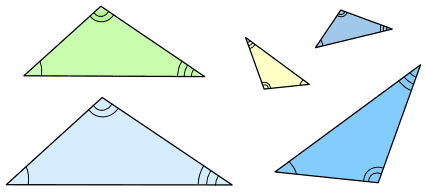
\includegraphics[width=\textwidth]{media/tri-similar1.png}
\end{frame}

\begin{frame}{Geometry of pinhole camera}
  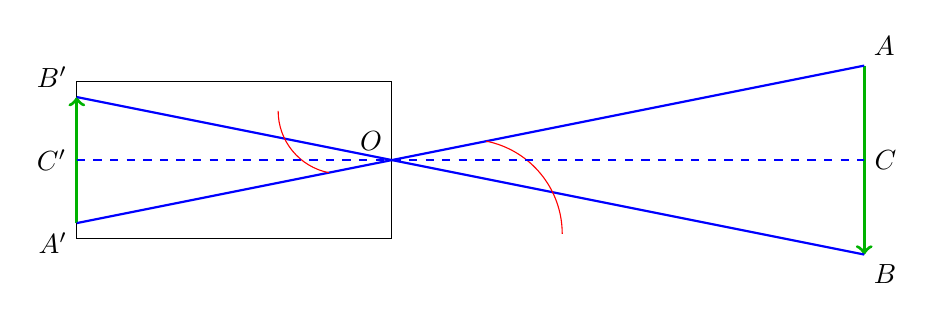
\begin{tikzpicture}
    \draw (-4,-1) rectangle (0, 1);
    \coordinate [label=above left:$O$] (origin) at (0,0);
    \coordinate [label=below left:$A'$] (imga) at (-4, -0.8);
    \coordinate [label=above left:$B'$] (imgb) at (-4, 0.8);
    \draw [->,very thick,green!70!black] (imga) -- (imgb);
    \coordinate [label=above right:$A$] (obja) at (6, 1.2);
    \coordinate [label=below right:$B$] (objb) at (6, -1.2);
    \draw [->,very thick,green!70!black] (obja) -- (objb);

    \draw [thick,blue] (imga) -- (obja);
    \draw [thick,blue] (imgb) -- (objb);
    
    \draw [red] let 
    \p1 = ($ 0.2*(imga) $),
    \n1 = {atan2(-\x1, -\y1)} 
    in (\x1,\y1) arc (\n1:0:\x1);

    \draw [red] let 
    \p1 = ($ 0.2*(obja) $),
    \n1 = {atan2(\x1, \y1)} 
    in (\x1,\y1) arc (\n1:0:\x1);

    \draw [thick,blue,dashed] ($0.5*(imga)+0.5*(imgb)$) node [text=black,anchor=east] {$C'$} -- ($0.5*(obja)+0.5*(objb)$) node [text=black,anchor=west] {$C$};
  \end{tikzpicture}
  \centering
  \begin{align}
    \frac{AC}{OC} &= \frac{A'C'}{OC'}\\
    \frac{\text{Size of object}}{\text{Distance of object}} &= \frac{\text{Size of screen}}{\text{Distance of image}}
  \end{align}
\end{frame}

\begin{frame}{Exercise}

  Can we compute the distance of object?\\
  \pause
  \begin{align}
    \text{Distance of object} = \frac{\text{Size of object}}{\text{Size of image}} \times \text{Distance of screen}
  \end{align}
\end{frame}

\begin{frame}{Distance and size of moon.}

  \begin{tikzpicture}
    \node [inner sep=0] (moonsmall) at (-3,0) {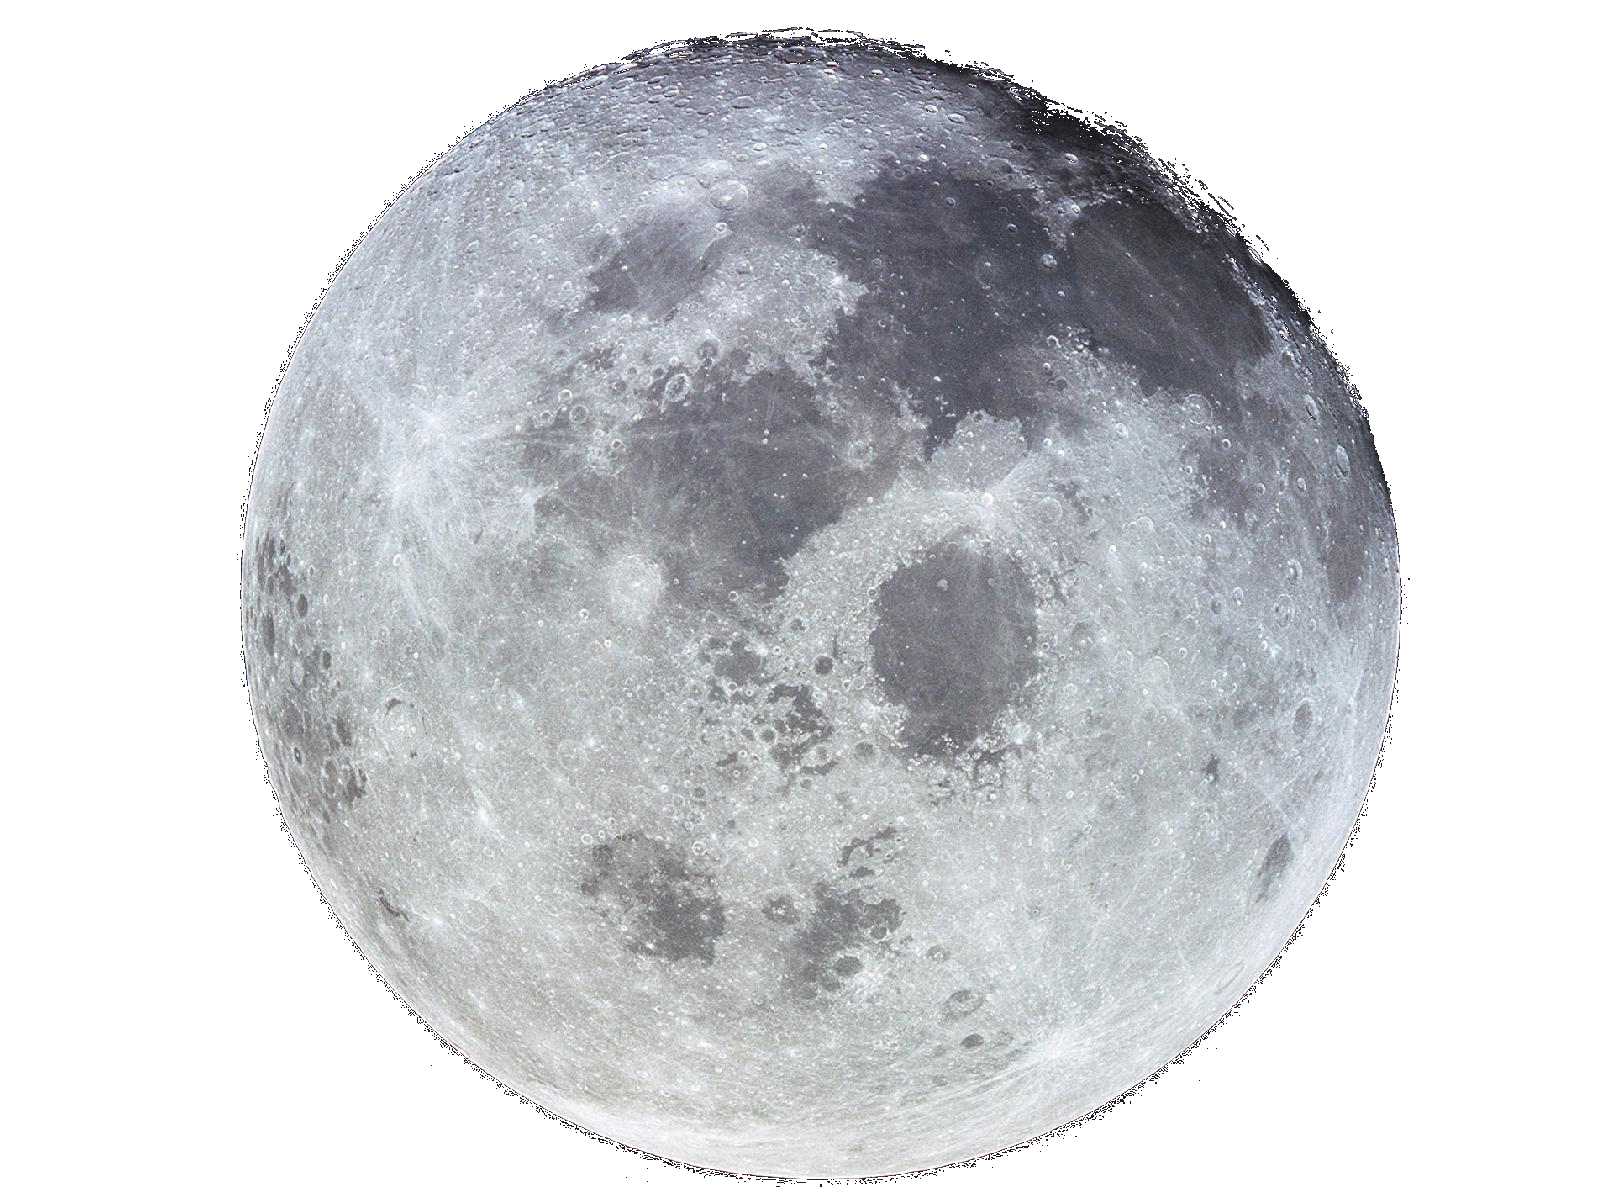
\includegraphics[height=1.5cm]{media/moon.png}};
    \node [inner sep=0] (moonlarge) at (-6,0) {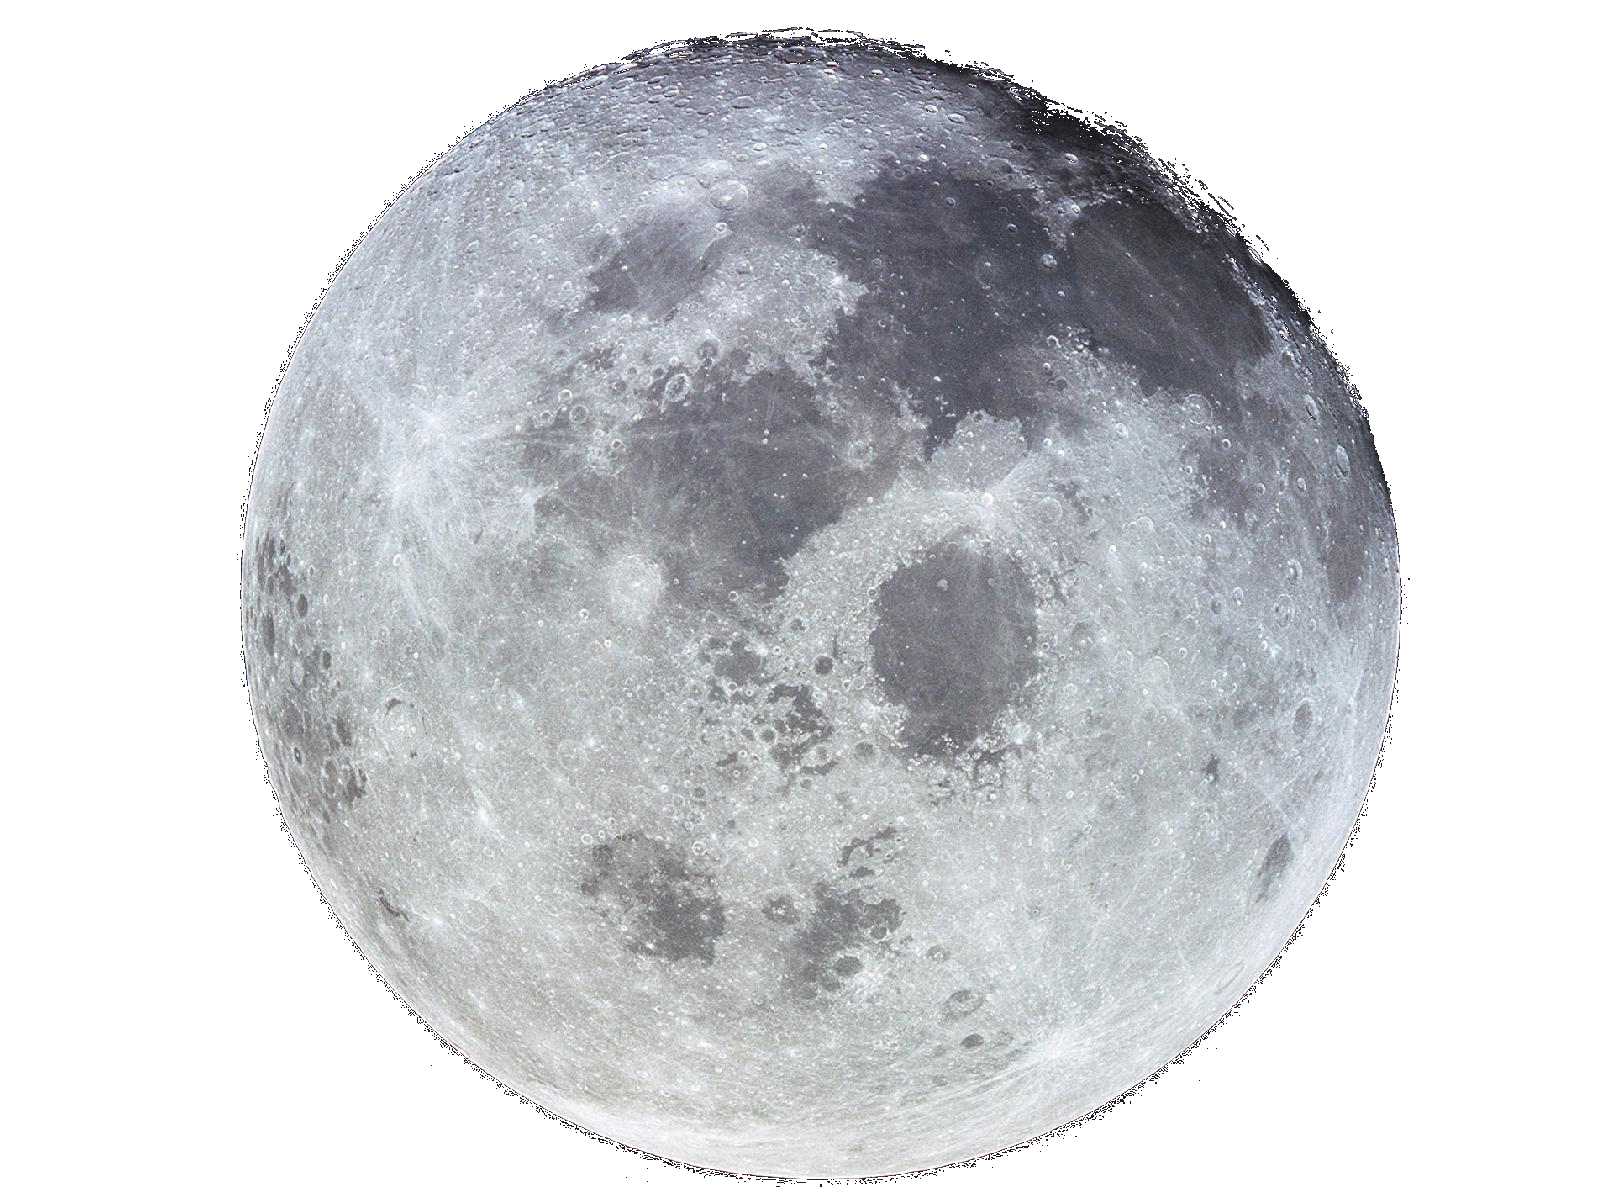
\includegraphics[height=3.0cm]{media/moon.png}};
    \node (eye) at (0,0) {
\includegraphics[height=1cm]{media/eye-left-viewing.png}};
    \draw (0,-1) rectangle (1,1);
    \node [inner sep=0] (moonimg) at (1,0) {\raisebox{\depth}{\scalebox{-1}[-1]{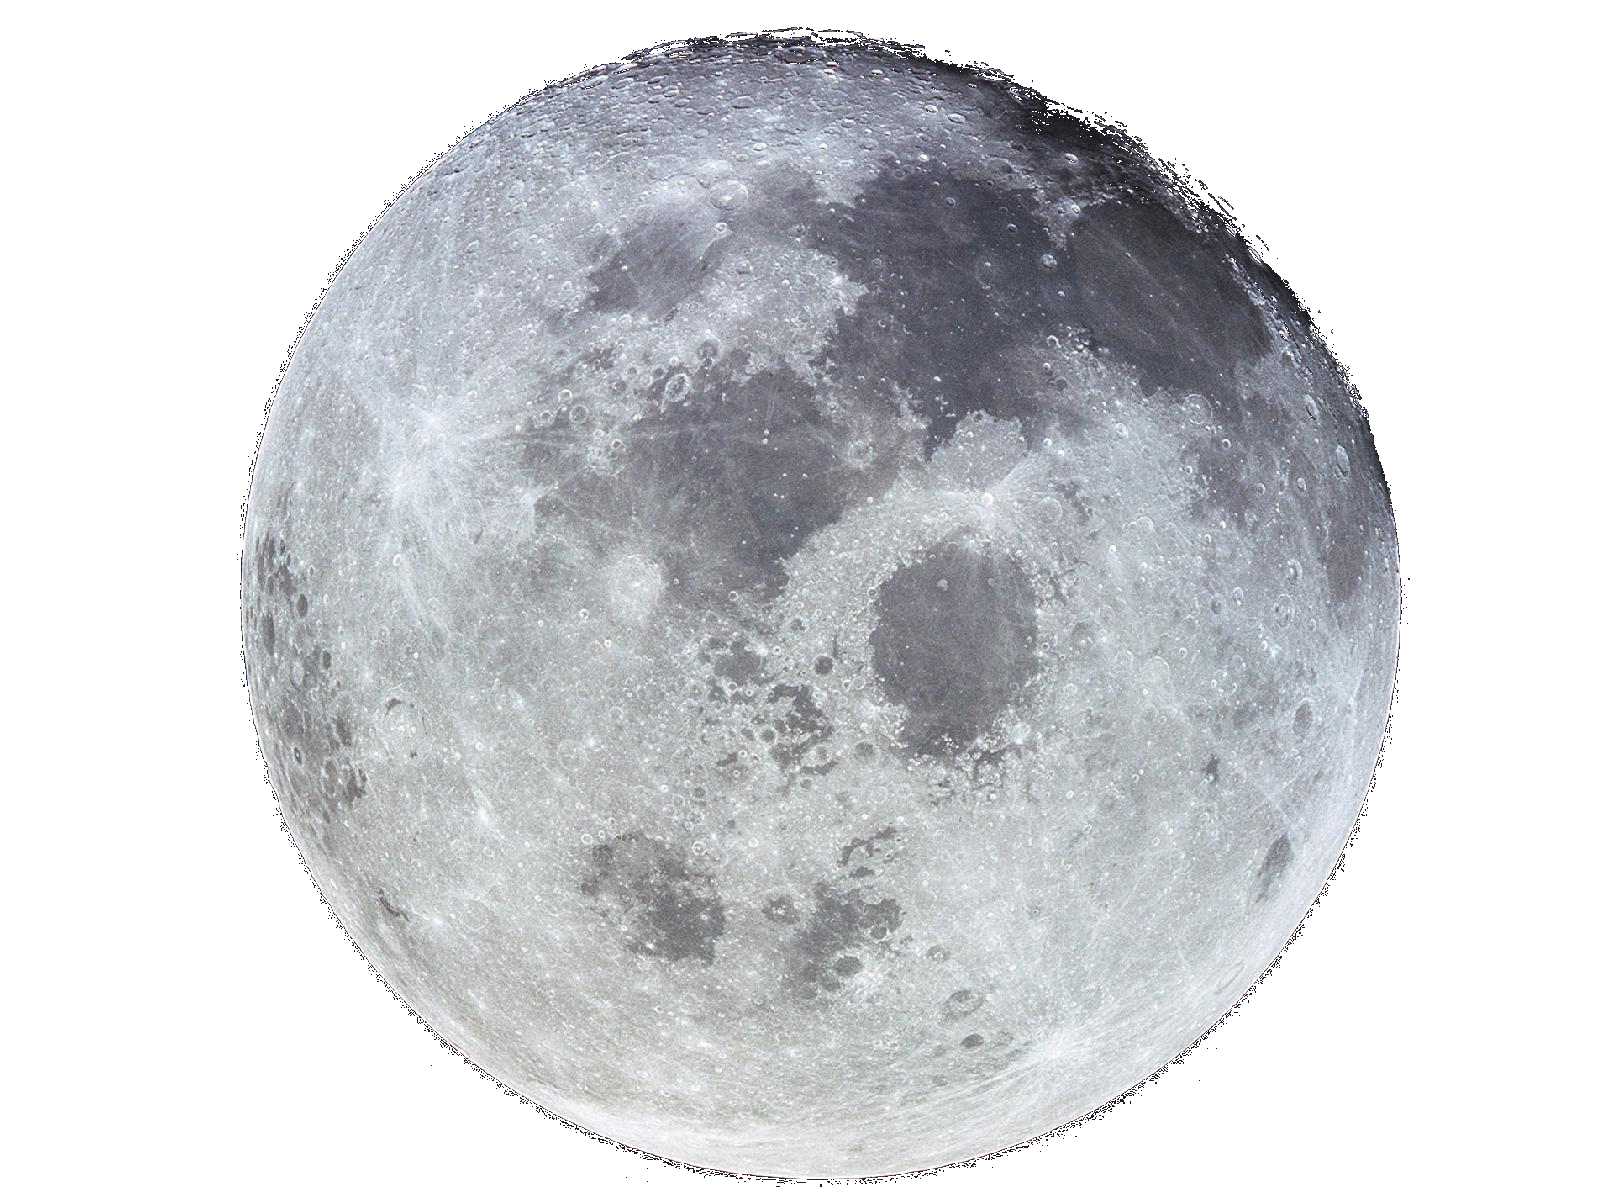
\includegraphics[height=.5cm]{media/moon.png}}}};
    \draw (moonimg.south) -- (moonlarge.north);
    \draw (moonimg.north) -- (moonlarge.south);
  \end{tikzpicture}
  \pause
  \\
  We CANNOT compute both the distance and size of moon from single image.
\end{frame}

\section{Effect of Aperture size}
\begin{frame}{Guess what happens?}
  ... if we make the pinhole a little bigger.\\
\end{frame}

\begin{frame}[fragile]{Scientific method}
  
             \newcommand{\textonecolor}[1]{\ifnum2<#1black\else black!50\fi}
  \only<2>{\renewcommand{\textonecolor}[1]{\ifnum3<##1black\else black!50\fi}}
  \only<4>{\renewcommand{\textonecolor}[1]{\ifnum4<##1black\else black!50\fi}}

             \newcommand{\nodeonecolor}[1]{\if3#1red!20\else none\fi}
  \only<2>{\renewcommand{\nodeonecolor}[1]{\if4##1red!20\else none\fi}}
  \only<4>{\renewcommand{\nodeonecolor}[1]{\if5##1red!20\else none\fi}}
  \begin{center}
    \begin{tikzpicture}[]

      \def \n {6}
      \def \radius {3}
      \def \margin {15} % margin in angles, depends on the radius

      \foreach \s/\t in {1/Purpose,2/Research,3/Hypothesis,4/Experiment,5/Analysis,6/Conclusion}
      {
        \node[fill=\nodeonecolor{\s},text=\textonecolor{\s},circle,minimum width=3] at ({360/\n * (\s - 1)}:\radius) {\t};
        \draw[->, >=latex] ({360/\n * (\s - 1)+\margin}:\radius) 
        arc ({360/\n * (\s - 1)+\margin}:{360/\n * (\s)-\margin}:\radius);
      }
    \end{tikzpicture}
    \addtooverlay<.(3)>{%
      \draw[fill=black,opacity=1.00] 
      (current page.north east) rectangle (current page.south west);
      \node at (current page.center) {
\includegraphics[height=\textheight]{media/tree.png}};
    }
  \end{center}

\end{frame}

\begin{frame}{Guess what happens?}
  ... if we make the pinhole a little bigger.\\
  \pause
  {\color{red} Image becomes brighter but blurred}
\end{frame}

\begin{frame}{Why?}
  \usetikzlibrary{calc}
\begin{tikzpicture}
\draw [very thick] (-2,-1) rectangle (0,1);
\fill [white] (-0.1,-0.08) rectangle (0.1,0.08);
\node [inner sep=-10] (tree) at (4,0) {
\includegraphics[height=4cm]{media/tree.png}};
\node [inner sep=-5](treeimg) at (-2,0) {\raisebox{\depth}{\scalebox{-1}[-1]{
\includegraphics[height=2cm]{media/tree.png}}}};
\draw [very thick] ($(tree.south)+(-.5,0.2)$) -- (treeimg.north);
\draw [very thick] ($(tree.north)+(-.5,-0.2)$) -- (treeimg.south);
\end{tikzpicture}
\\
  \usetikzlibrary{calc}
\begin{tikzpicture}
\draw [very thick] (-2,-1) rectangle (0,1);
\fill [white] (-0.1,-0.2) rectangle (0.1,0.2);
\node [inner sep=-10] (tree) at (4,0) {
\includegraphics[height=4cm]{media/tree.png}};
\node [inner sep=-5](treeimg1) at (-2,0.2) {\raisebox{\depth}{\scalebox{-1}[-1]{
\includegraphics[height=2cm]{media/tree.png}}}};
\draw [very thick] ($(tree.south)+(-.5,0.2)$)-- (treeimg1.north);
\draw [very thick] ($(tree.north)+(-.5,-0.2)$) -- (treeimg1.south);


\node [inner sep=-5](treeimg2) at (-2,-0.2) {\raisebox{\depth}{\scalebox{-1}[-1]{
\includegraphics[height=2cm]{media/tree.png}}}};

\draw [very thick] ($(tree.south)+(-.5,0.2)$) -- (treeimg2.north);
\draw [very thick] ($(tree.north)+(-.5,-0.2)$) -- (treeimg2.south);
\end{tikzpicture}

\end{frame}

\begin{frame}{Fun fact!!}
  \begin{center}
    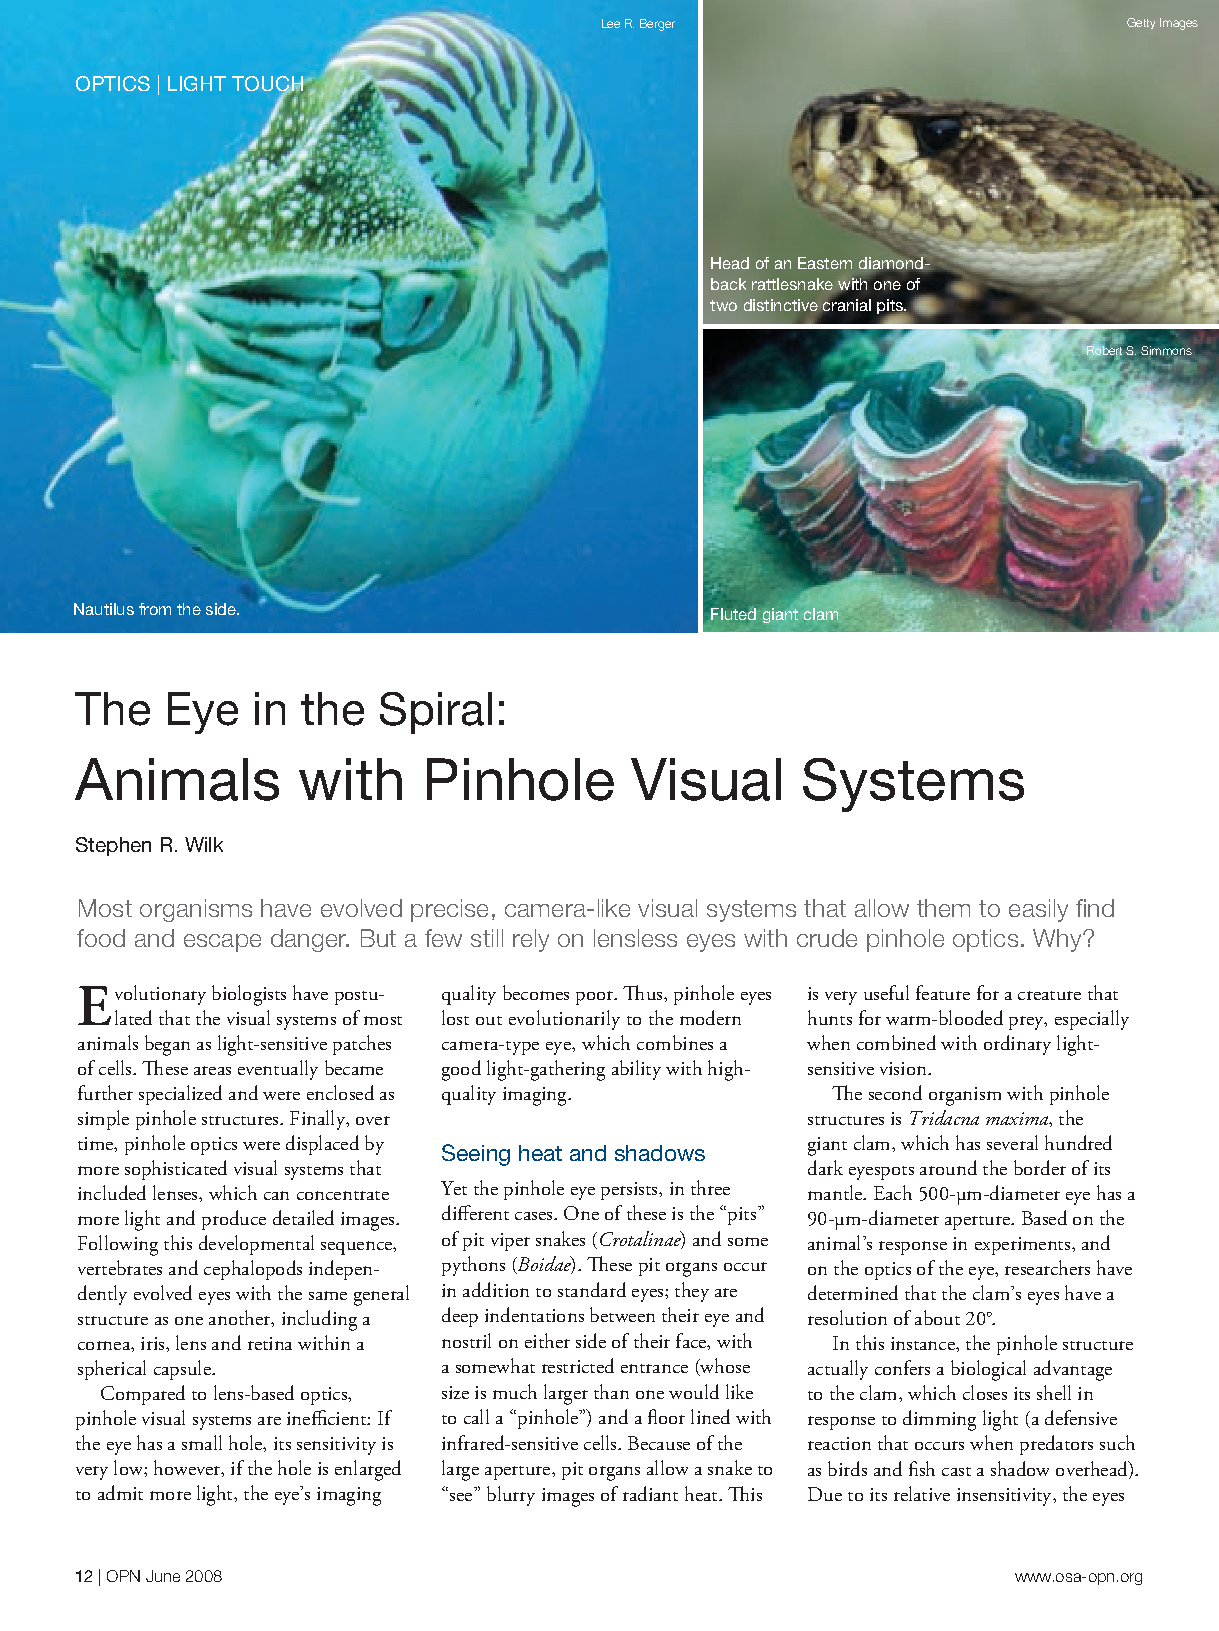
\includegraphics[width=0.8\textwidth, trim=0 5in 0 0,clip]{media/animalspinhole.pdf}
  \end{center}
\end{frame}
\begin{frame}
  \begin{center}
    \includemedia[label=chambered-nautilus-accident,
      width=\linewidth,height=0.6\linewidth, % 16:9
      activate=pageopen,
      addresource=media/chambered-nautilus-accident.mp4,
      flashvars={
        source=media/chambered-nautilus-accident.mp4
        &loop=false             % loop video
        &scaleMode=letterbox   % preserve aspect ratio while scaling the video
      }
    ]{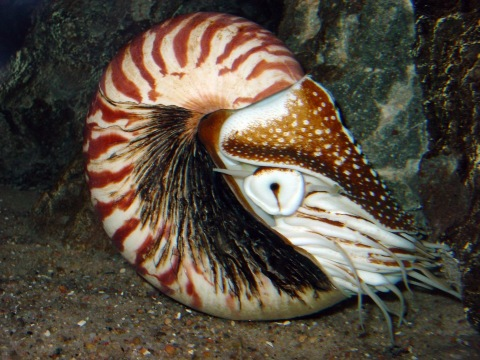
\includegraphics{media/chambered-nautilus-accident.jpg}}{VPlayer.swf}
  \end{center}
\end{frame}

\section{Number of Apertures}
\begin{frame}{Guess what happens}
  ... if we make multiple holes around the pinhole?\\
\end{frame}

\begin{frame}[fragile]{Scientific method}
  
             \newcommand{\textonecolor}[1]{\ifnum2<#1black\else black!50\fi}
  \only<2>{\renewcommand{\textonecolor}[1]{\ifnum3<##1black\else black!50\fi}}
  \only<4>{\renewcommand{\textonecolor}[1]{\ifnum4<##1black\else black!50\fi}}

             \newcommand{\nodeonecolor}[1]{\if3#1red!20\else none\fi}
  \only<2>{\renewcommand{\nodeonecolor}[1]{\if4##1red!20\else none\fi}}
  \only<4>{\renewcommand{\nodeonecolor}[1]{\if5##1red!20\else none\fi}}
  \begin{center}
    \begin{tikzpicture}[]

      \def \n {6}
      \def \radius {3}
      \def \margin {15} % margin in angles, depends on the radius

      \foreach \s/\t in {1/Purpose,2/Research,3/Hypothesis,4/Experiment,5/Analysis,6/Conclusion}
      {
        \node[fill=\nodeonecolor{\s},text=\textonecolor{\s},circle,minimum width=3] at ({360/\n * (\s - 1)}:\radius) {\t};
        \draw[->, >=latex] ({360/\n * (\s - 1)+\margin}:\radius) 
        arc ({360/\n * (\s - 1)+\margin}:{360/\n * (\s)-\margin}:\radius);
      }
    \end{tikzpicture}
    \addtooverlay<.(3)>{%
      \draw[fill=black,opacity=1.00] 
      (current page.north east) rectangle (current page.south west);
      \node at (current page.center) {
\includegraphics[height=\textheight]{media/tree.png}};
    }
  \end{center}

\end{frame}

\begin{frame}{Guess what happens}
  ... if we make multiple holes around the pinhole?\\
  \pause
  {\color{red} Did you get multiple images?}
\end{frame}

\begin{frame}{Evolution of eye}

                \newcommand{\overlayhide}{\fill [white,opacity=0.8] (0,0) -- (0,0.65) --(0.55,0.65) --  (0.55, 1.0) -- (1,1) -- (1,0) -- cycle;}
    \only<2->{\renewcommand{\overlayhide}{\fill [white,opacity=0.8] (0,0) -- (0,0.65) --(0.55,0.65) --  (0.55, 0.65) -- (1,0.65) -- (1,0) -- cycle;}}
    \only<3->{\renewcommand{\overlayhide}{\fill [white,opacity=0.8] (0,0) -- (0,0.33) --(0.50,0.33) --  (0.50, 0.65) -- (1,0.65) -- (1,0) -- cycle;}}
    \only<4->{\renewcommand{\overlayhide}{\fill [white,opacity=0.8] (0,0) -- (0,0.33) --(0.50,0.33) --  (0.50, 0.33) -- (1,0.33) -- (1,0) -- cycle;}}
    \only<5->{\renewcommand{\overlayhide}{\fill [white,opacity=0.8] (0,0) -- (0,0.00) --(0.50,0.00) --  (0.50, 0.33) -- (1,0.33) -- (1,0) -- cycle;}}
    \only<6->{\renewcommand{\overlayhide}{\fill [white,opacity=0.8] (0,0) -- (0,0.00) --(0.50,0.00) --  (0.50, 0.00) -- (1,0.00) -- (1,0) -- cycle;}}
  \begin{center}

    \begin{tikzpicture}
      \node [anchor=south west,inner sep=0](img) at (0,0) {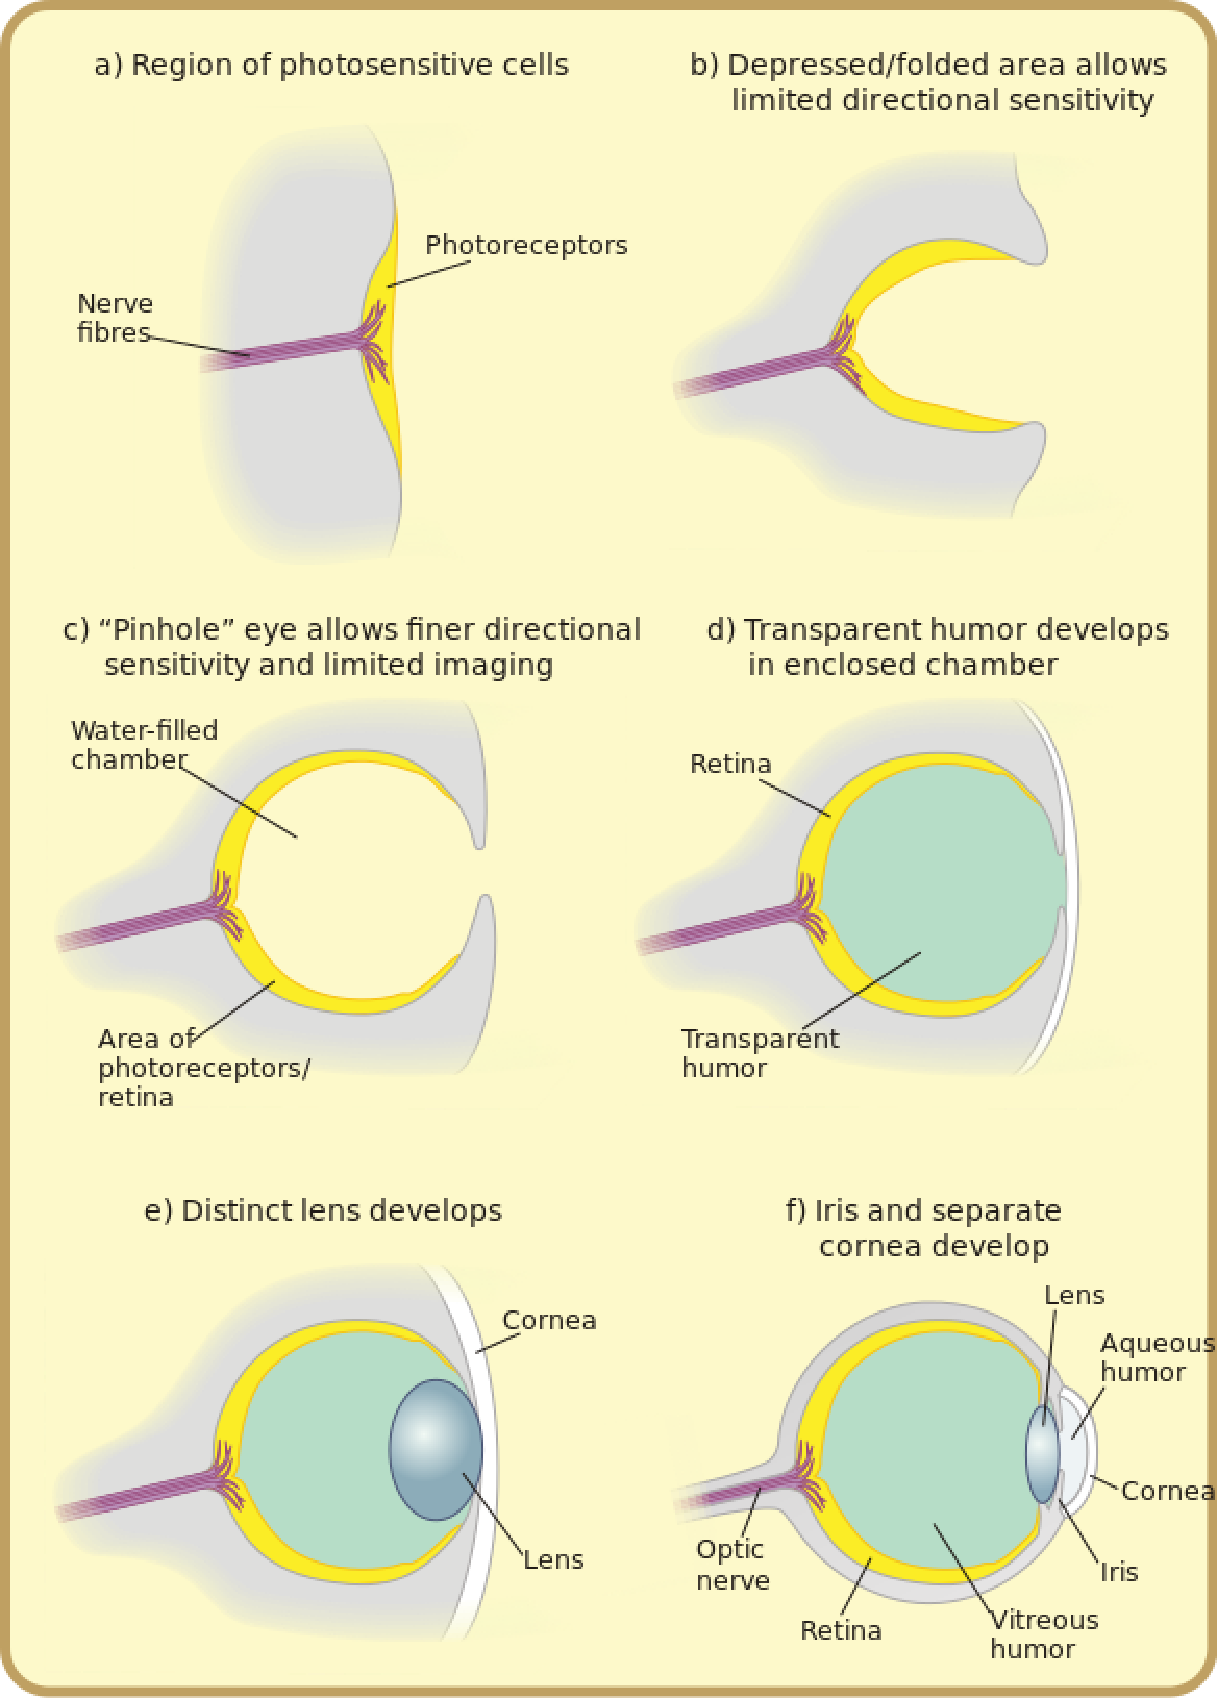
\includegraphics[height=0.8\textheight]{media/Diagram_of_eye_evolution.pdf}};
      \begin{scope}[x={(img.south east)},y={(img.north west)}]
        \overlayhide
      \end{scope}
    \end{tikzpicture}
  \end{center}
\end{frame}

\begin{frame}{Introducing lens}
  We want to find out a lens that will make our camera better.
\end{frame}

\begin{frame}[fragile]{Scientific method}
  
             \newcommand{\textonecolor}[1]{\ifnum2<#1black\else black!50\fi}
  \only<2>{\renewcommand{\textonecolor}[1]{\ifnum3<##1black\else black!50\fi}}
  \only<4>{\renewcommand{\textonecolor}[1]{\ifnum4<##1black\else black!50\fi}}

             \newcommand{\nodeonecolor}[1]{\if3#1red!20\else none\fi}
  \only<2>{\renewcommand{\nodeonecolor}[1]{\if4##1red!20\else none\fi}}
  \only<4>{\renewcommand{\nodeonecolor}[1]{\if5##1red!20\else none\fi}}
  \begin{center}
    \begin{tikzpicture}[]

      \def \n {6}
      \def \radius {3}
      \def \margin {15} % margin in angles, depends on the radius

      \foreach \s/\t in {1/Purpose,2/Research,3/Hypothesis,4/Experiment,5/Analysis,6/Conclusion}
      {
        \node[fill=\nodeonecolor{\s},text=\textonecolor{\s},circle,minimum width=3] at ({360/\n * (\s - 1)}:\radius) {\t};
        \draw[->, >=latex] ({360/\n * (\s - 1)+\margin}:\radius) 
        arc ({360/\n * (\s - 1)+\margin}:{360/\n * (\s)-\margin}:\radius);
      }
    \end{tikzpicture}
    \addtooverlay<.(3)>{%
      \draw[fill=black,opacity=1.00] 
      (current page.north east) rectangle (current page.south west);
      \node at (current page.center) {
\includegraphics[height=\textheight]{media/tree.png}};
    }
  \end{center}

\end{frame}

\begin{frame}{Introducing lens}
  Add the double convex lens in front of multiple pinholes?\\
  \pause
  Do you see all images merging into one?\\
  What happened?
\end{frame}

\begin{frame}{Understanding refraction}
  \centering
  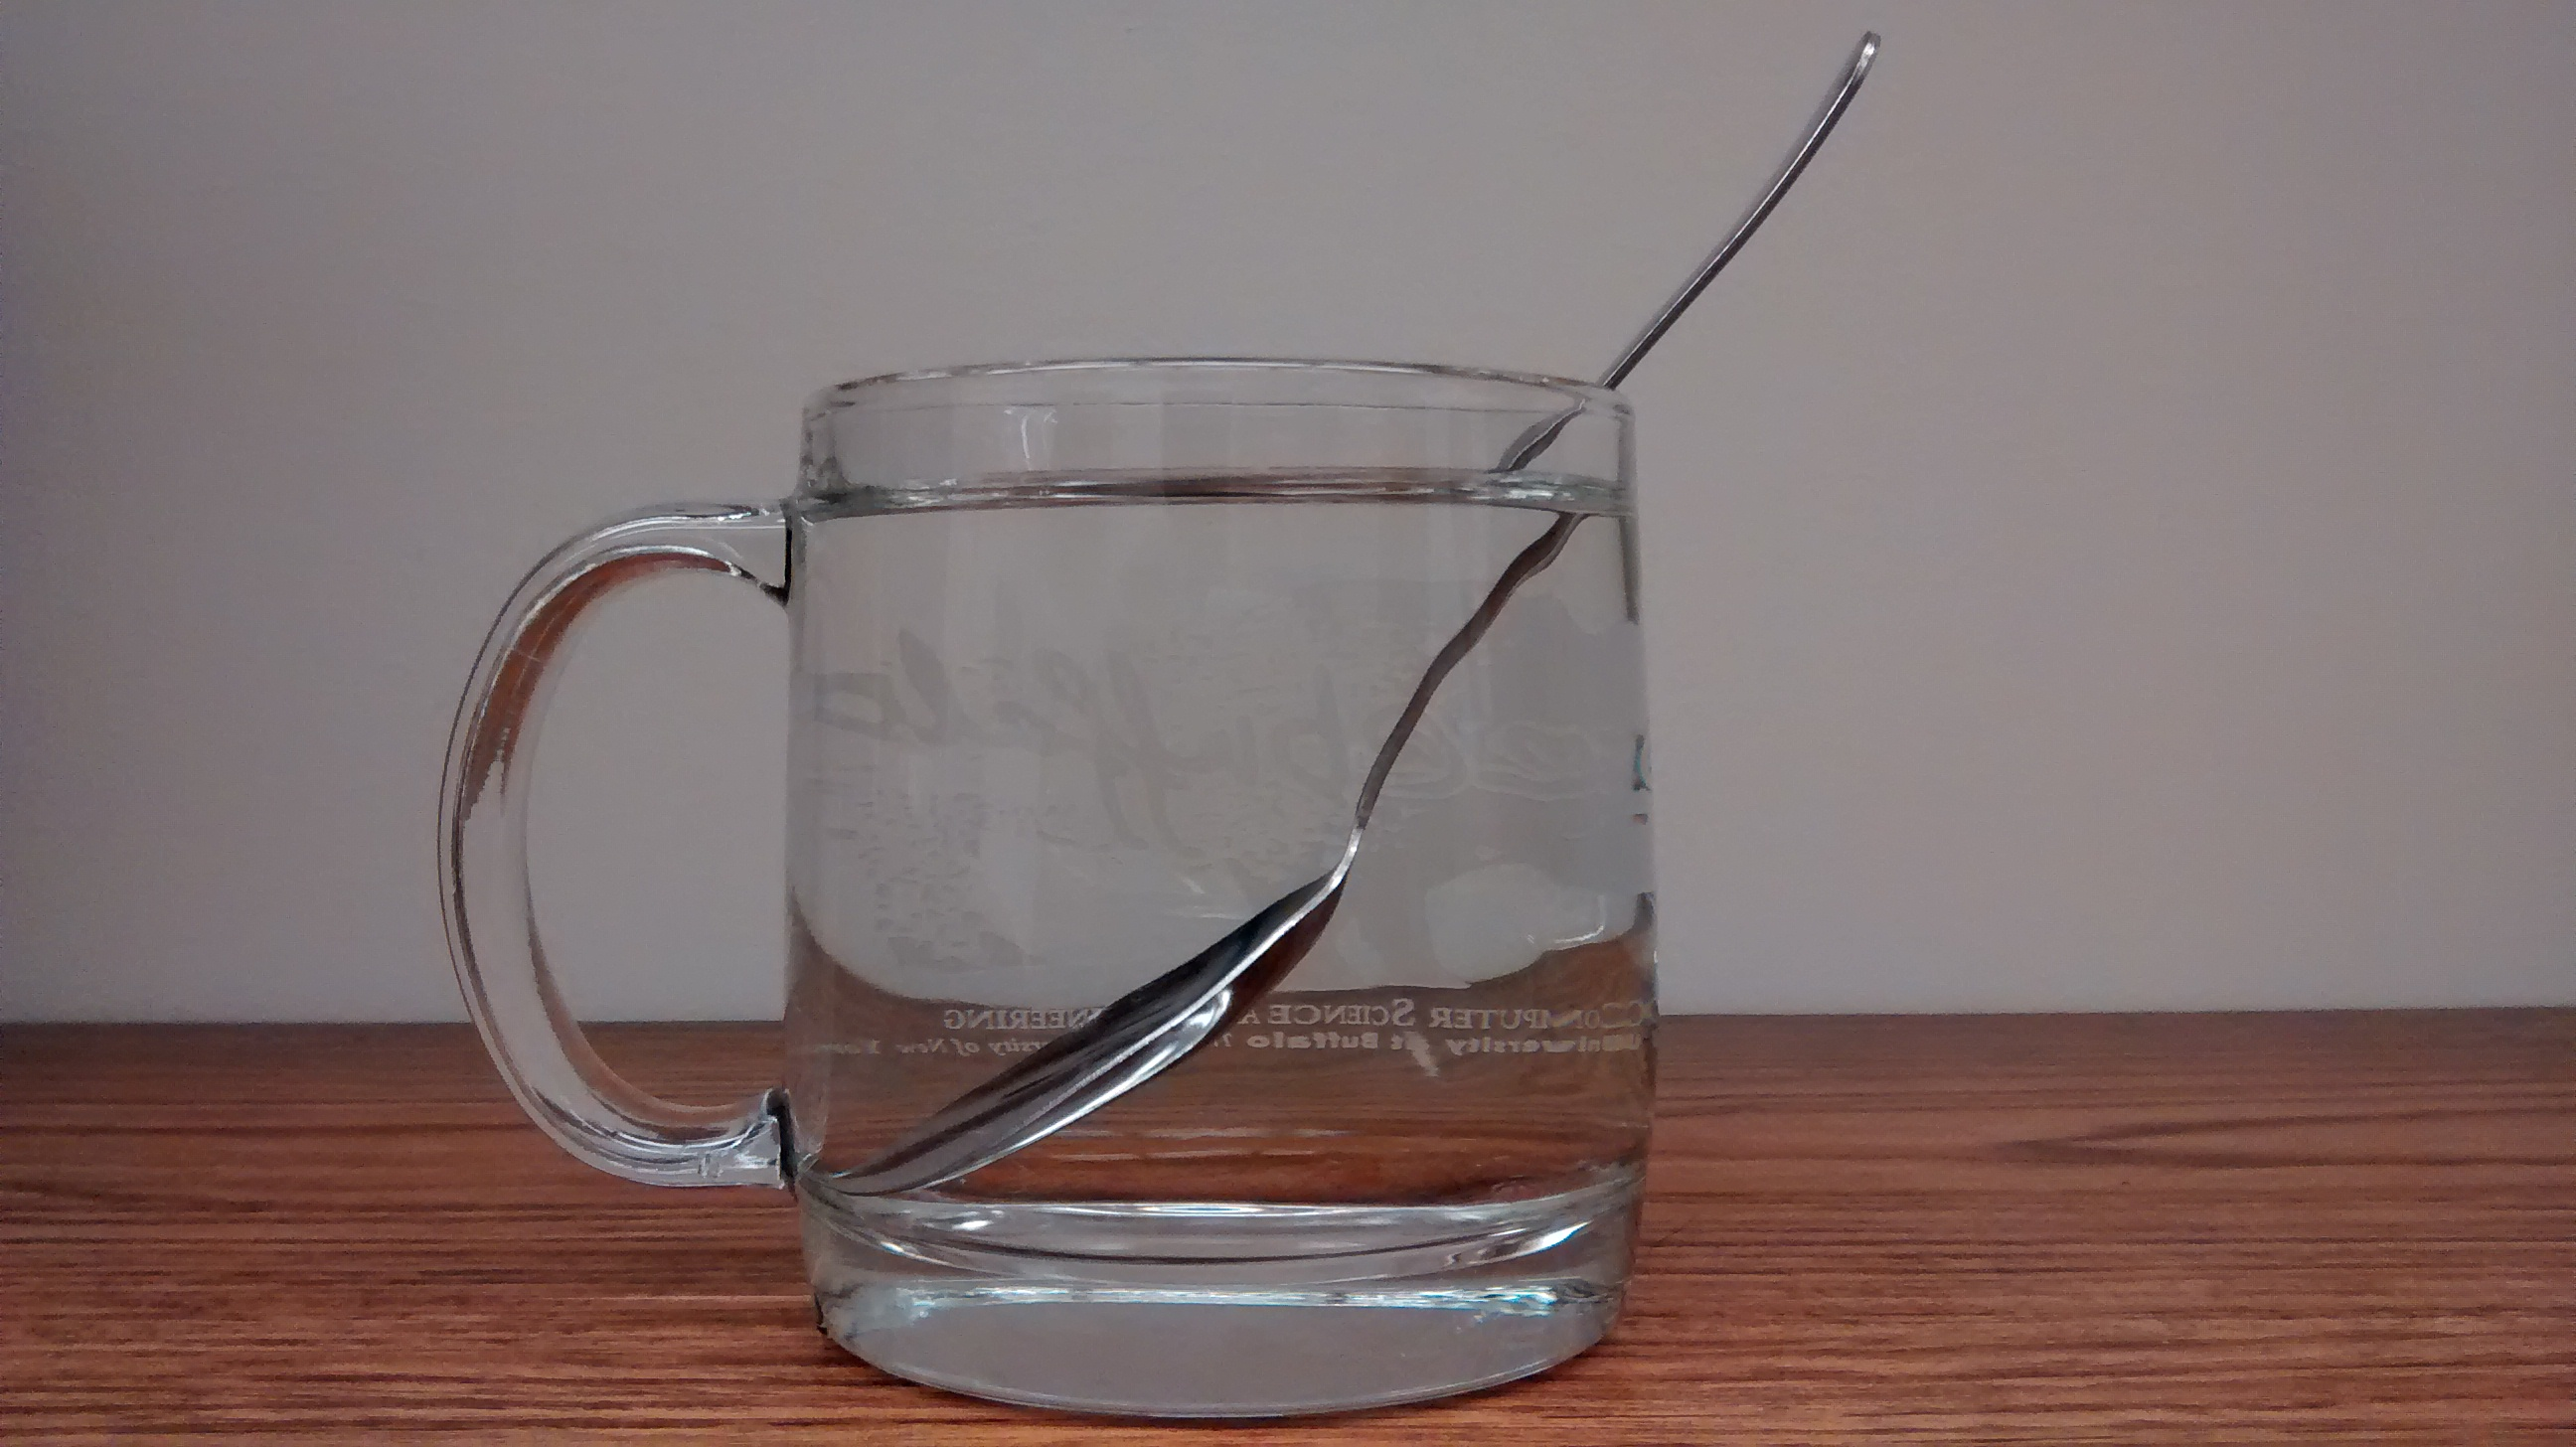
\includegraphics[width=\textwidth]{media/refractionspoon.jpg}
\end{frame}

\begin{frame}{Refraction}
  Light bends towards normal when enters a denser medium \\
  \visible<2->{
  Light bends away from normal when enters a lighter medium}
  \begin{center}
    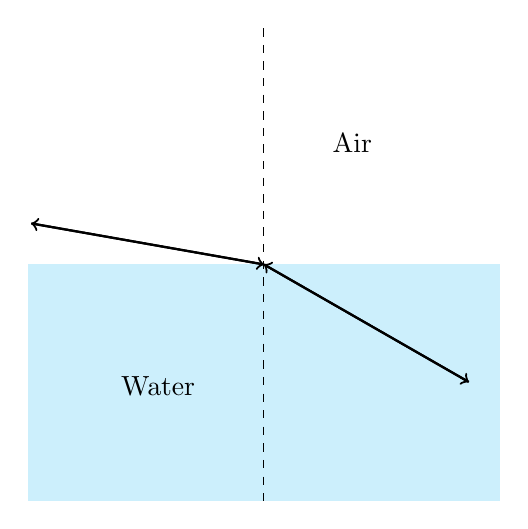
\begin{tikzpicture}[scale=3.0]
      \fill [cyan!20!white] (-1,-1) rectangle (1,0);
      \draw [dashed] (90:1) -- (-90:1);
      \visible<-1>{
        \draw [->,thick] (170:1) -- (0,0);
        \draw [->,thick] (0,0) -- (-29.84:1);
      }
      \visible<2->{
        \draw [<-,thick] (170:1) -- (0,0);
        \draw [<-,thick] (0,0) -- (-29.84:1);
      }
      \node at (60:0.5) [anchor=south west] {Air};
      \node at (-120:0.5) [anchor=north east] {Water};
    \end{tikzpicture}
  \end{center}
\end{frame}

\begin{frame}{Refraction in nature}
  Twinkling starts\\
  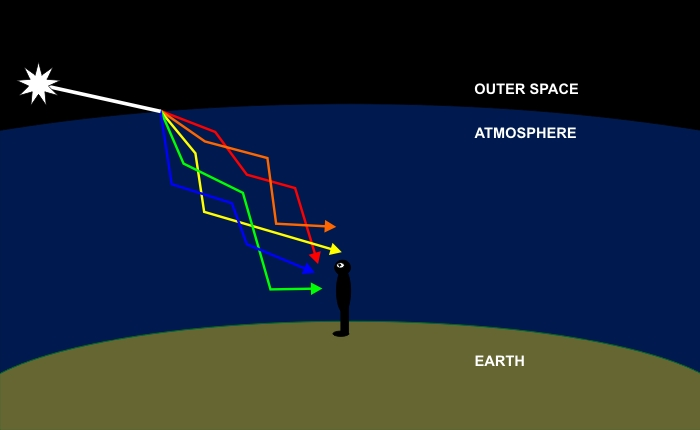
\includegraphics[width=\textwidth]{media/twinkle.jpg}
\end{frame}
\begin{frame}{Refraction in nature}
  Longer days\\
  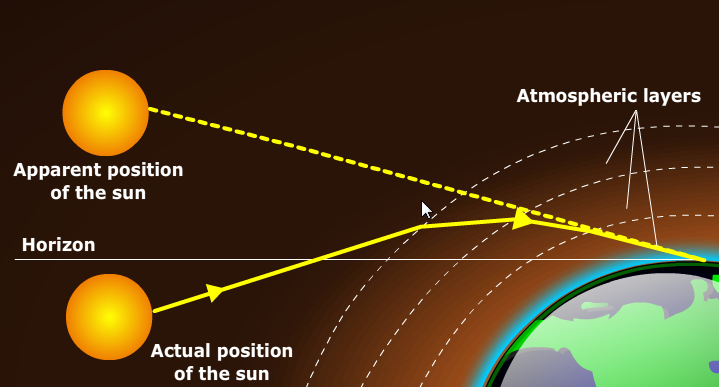
\includegraphics[width=\textwidth]{media/sunset.png}
\end{frame}

\begin{frame}{Refraction}
  Light bends towards normal when enters a denser medium
  \begin{center}
    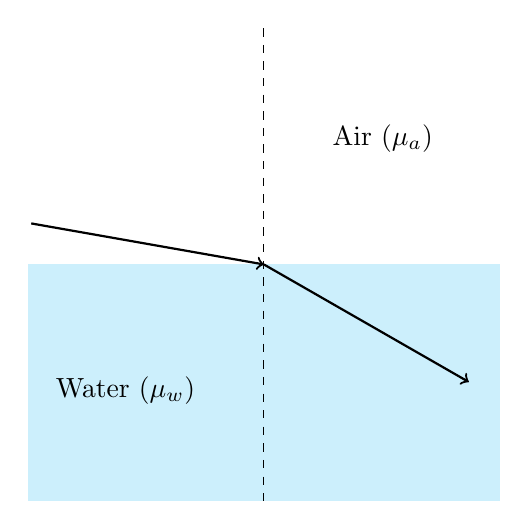
\begin{tikzpicture}[scale=3.0]
      \fill [cyan!20!white] (-1,-1) rectangle (1,0);
      \draw [dashed] (90:1) -- (-90:1);
      \draw [->,thick] (170:1) -- (0,0);
      \draw [->,thick] (0,0) -- (-29.84:1);
      \node at (60:0.5) [anchor=south west] {Air ($\mu_a$)};
      \node at (-120:0.5) [anchor=north east] {Water ($\mu_w$)};
    \end{tikzpicture}
  \end{center}
\end{frame}

\begin{frame}{Refraction at lens}
  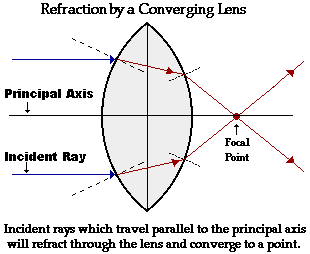
\includegraphics[height=0.8\textheight]{media/convexlens.png}
\end{frame}

\begin{frame}{Interactive animation}

  \url{http://www.pbslearningmedia.org/resource/lsps07.sci.phys.energy.geometoptics/geometric-optics/}

\end{frame}
\end{document}
